\chapter{Testing}\label{Testing}
A prototype or proof-of-concept can be difficult to use as a selling point, without proof that the product works. Scheduling tests for different parameters of the product can help improve the credibility by showing that different parts of the product works and documenting the strengths and weaknesses of it.


\section{LIDAR Accuracy test}
Testing the equipment of the system is important, as it may impact how the system functions as a whole. This test will test the error margin of the LIDARs, by reading the distance from the LIDAR to the distance of an object.\\

\textbf{Equipment}: The equipment used is a SICK TiM571 LIDAR, measuring tape, a cardboard and software to read distances measured from the LIDAR.\\
    
\textbf{Setup}: The LIDAR is placed in a corner with 5 meters of free space in a 10 degree angle. This is to help leave out the things the LIDAR should not be measuring distance to. Lines were drawn on the floor that had a distance relative to the middle of the LIDAR, as if the LIDAR was placed on the floor (currently it is mounted on the robot). Two people, person A and person B have each their job. Person A holds a piece of cardboard that is placed orthogonal to the LIDAR, see on figure \ref{fig:AccuracySetup1}, on the marked spots that had a distance of 0.5m, 1m, 1.5m, 2m, 2.5m, 3m, 3.5m, 4m, 4.5m relative to the LIDAR, see figure \ref{fig:AccuracySetup2}. Person B has to read the distance, information read on the computer that comes from the LIDAR software.

\begin{figure}[H]
    \centering
    \begin{minipage}[b]{0.5\linewidth}
        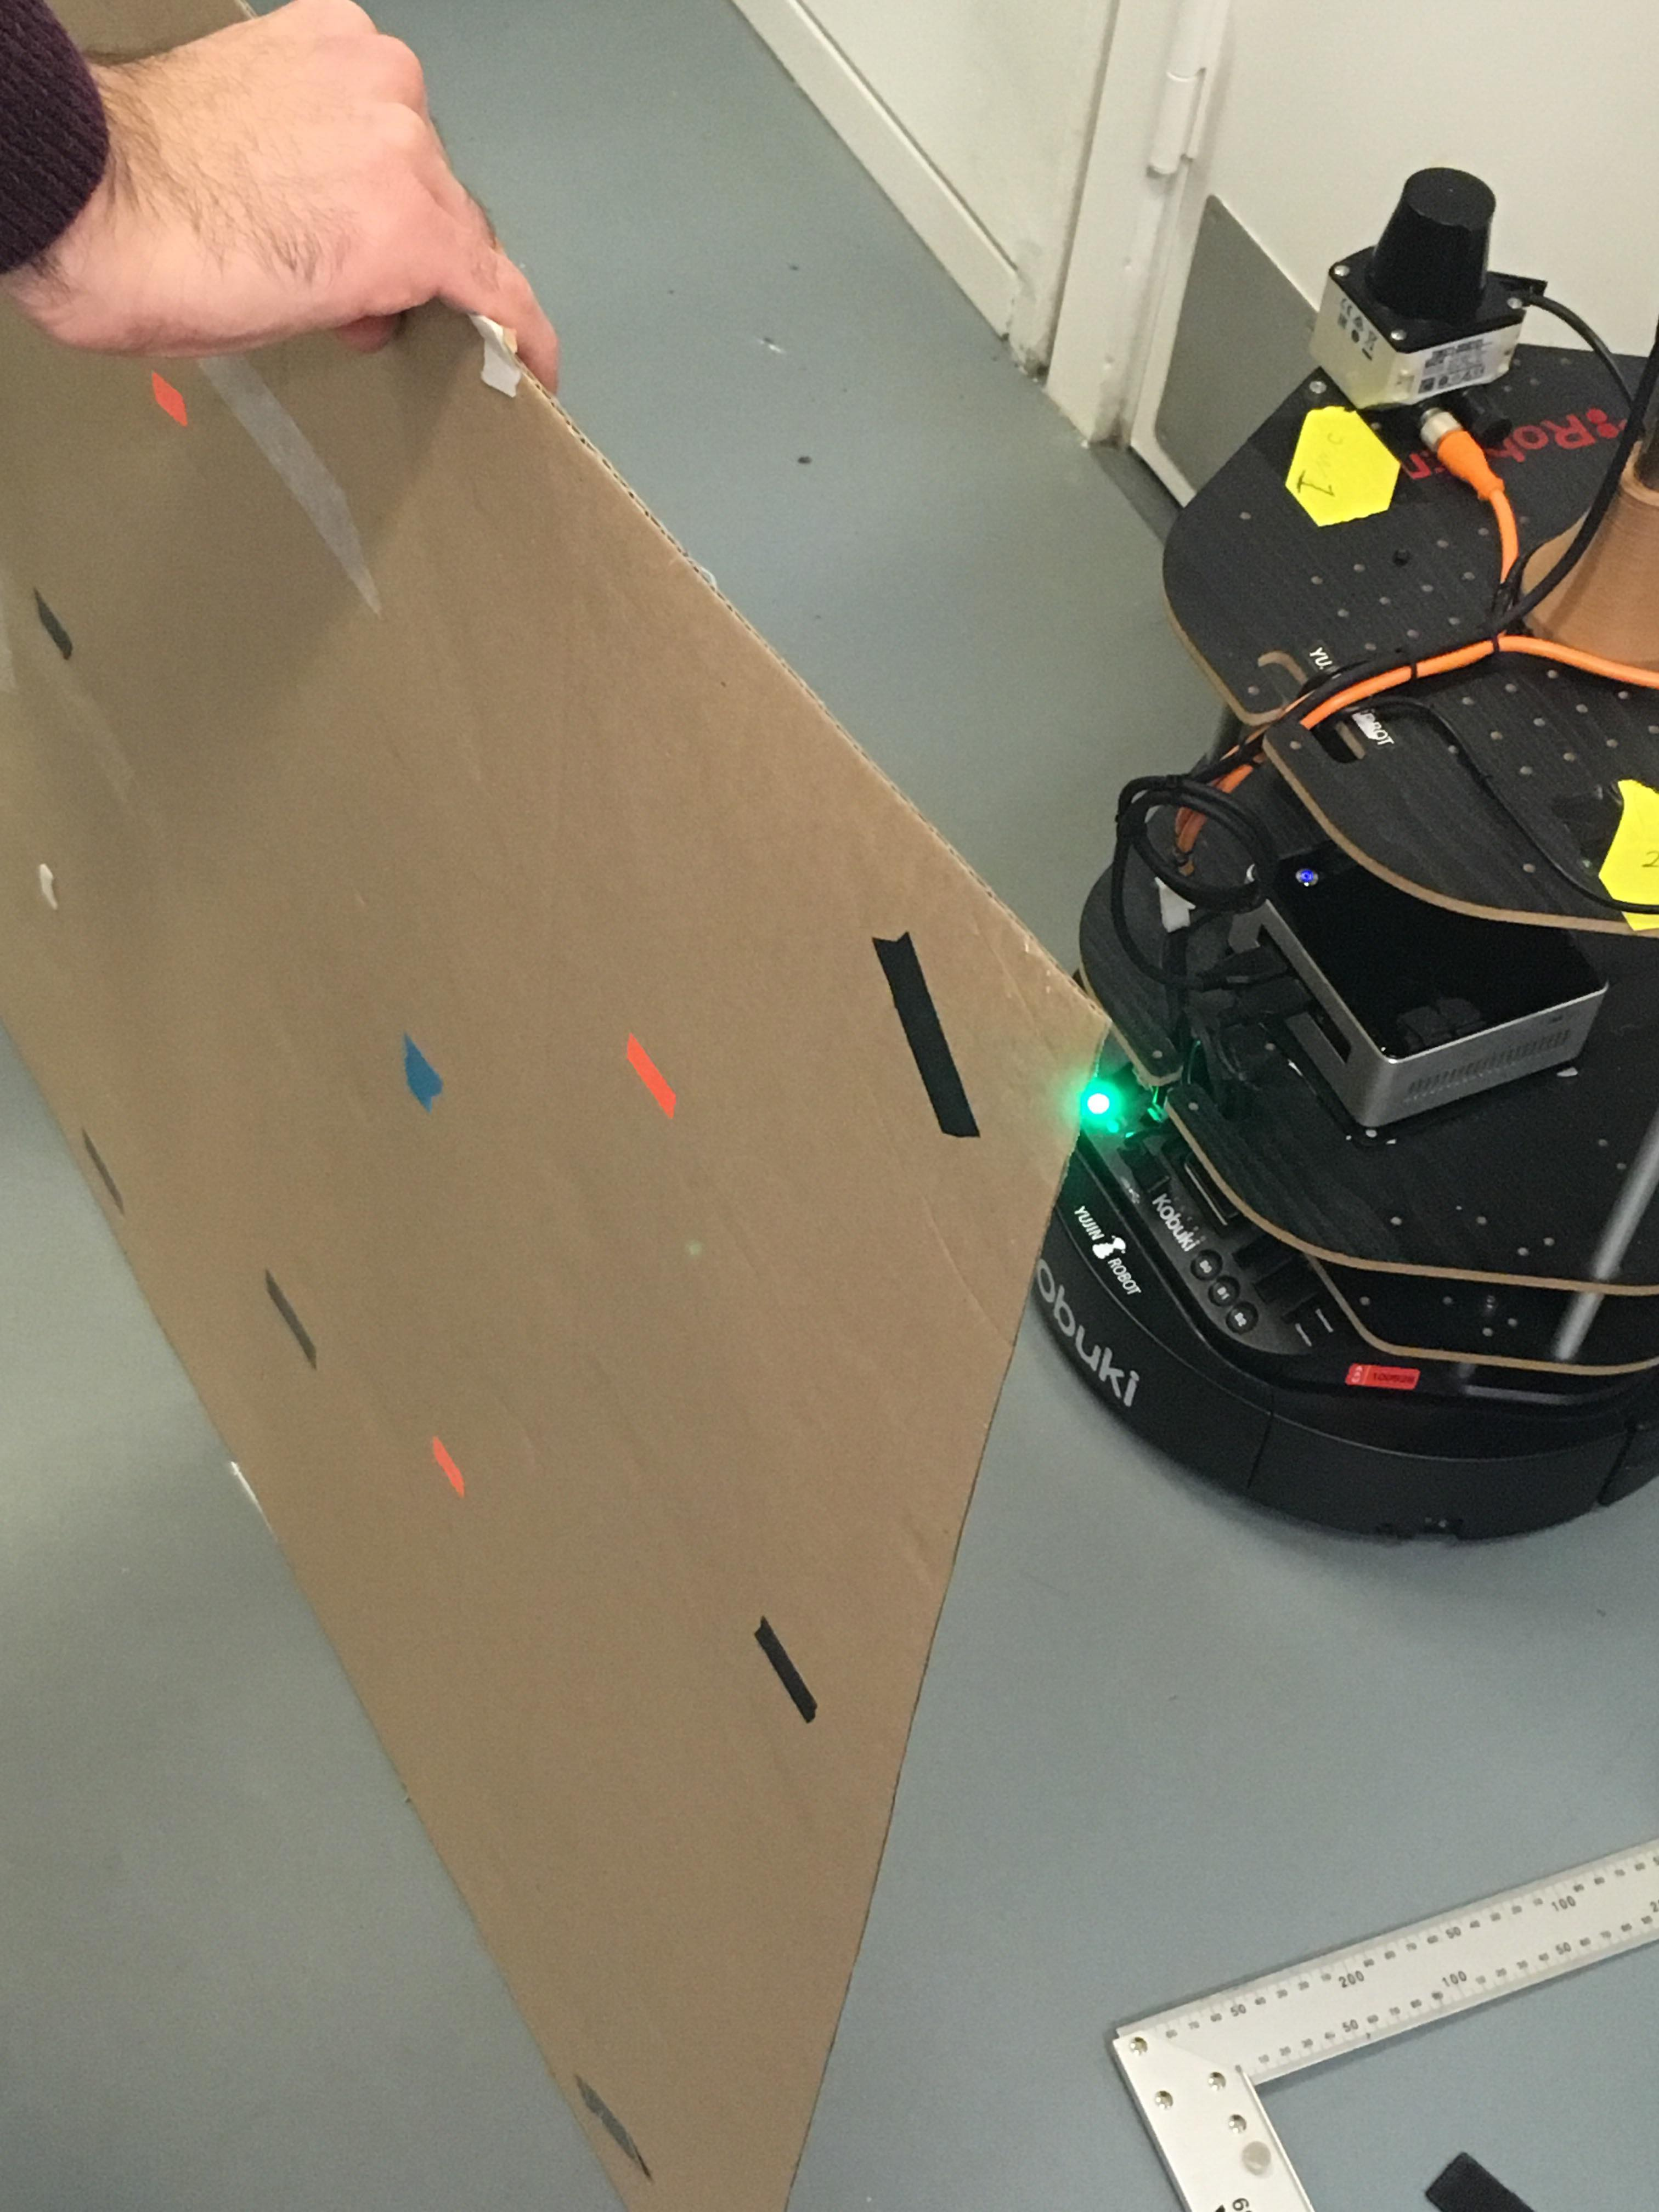
\includegraphics[width=\textwidth]{figures/AccuracySetup1.jpg}
        \caption{Person A holding the cardboard piece at a distance of 0.5m from the LIDAR. The 0.5m mark made with the white chalk is barely visible at the bottom of the board.}
        \label{fig:AccuracySetup1}
    \end{minipage}
    \hspace{0.2cm}
    \begin{minipage}[b]{0.45\linewidth}
        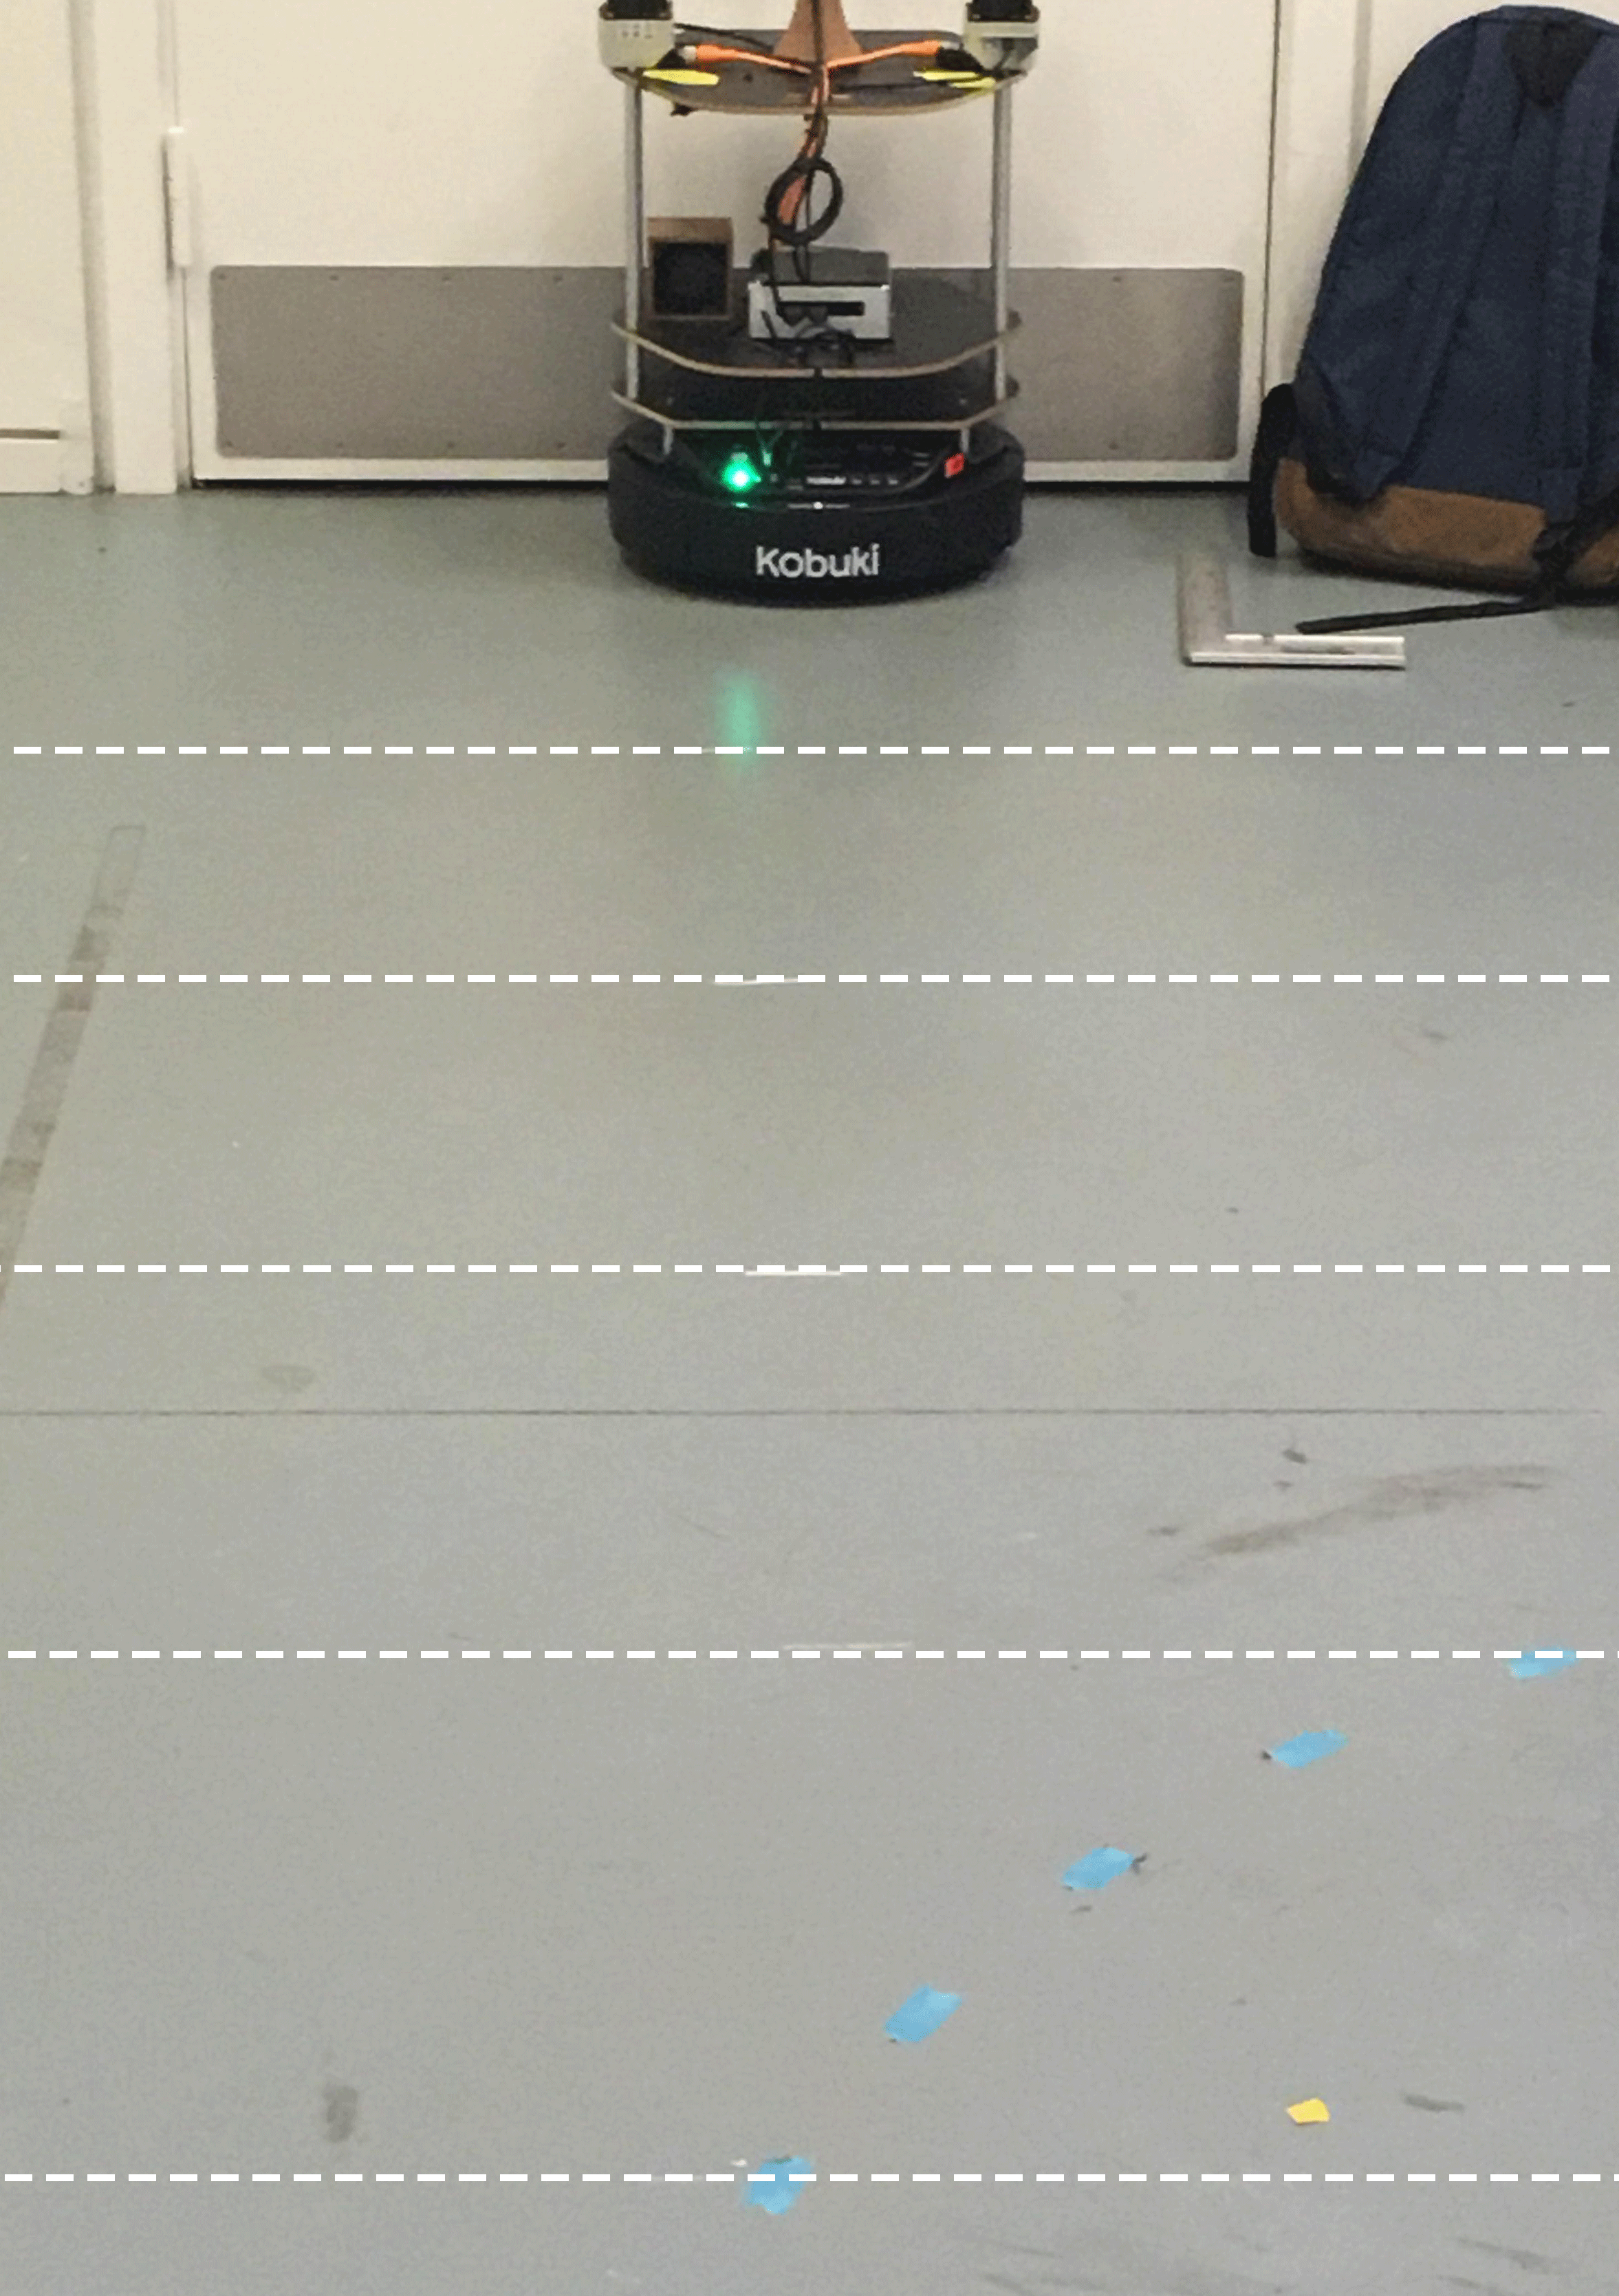
\includegraphics[width=\textwidth]{figures/AccuracySetupPs.png}
        \caption{The position of the robot and LIDAR, with white spotted lines placed on top  of the chalk lines that have been drawn on the floor, marking the distance to the LIDAR with an increment of 0.5m for each line.}
        \label{fig:AccuracySetup2}
    \end{minipage}
\end{figure}

% \begin{figure}[H]
%     \centering
%     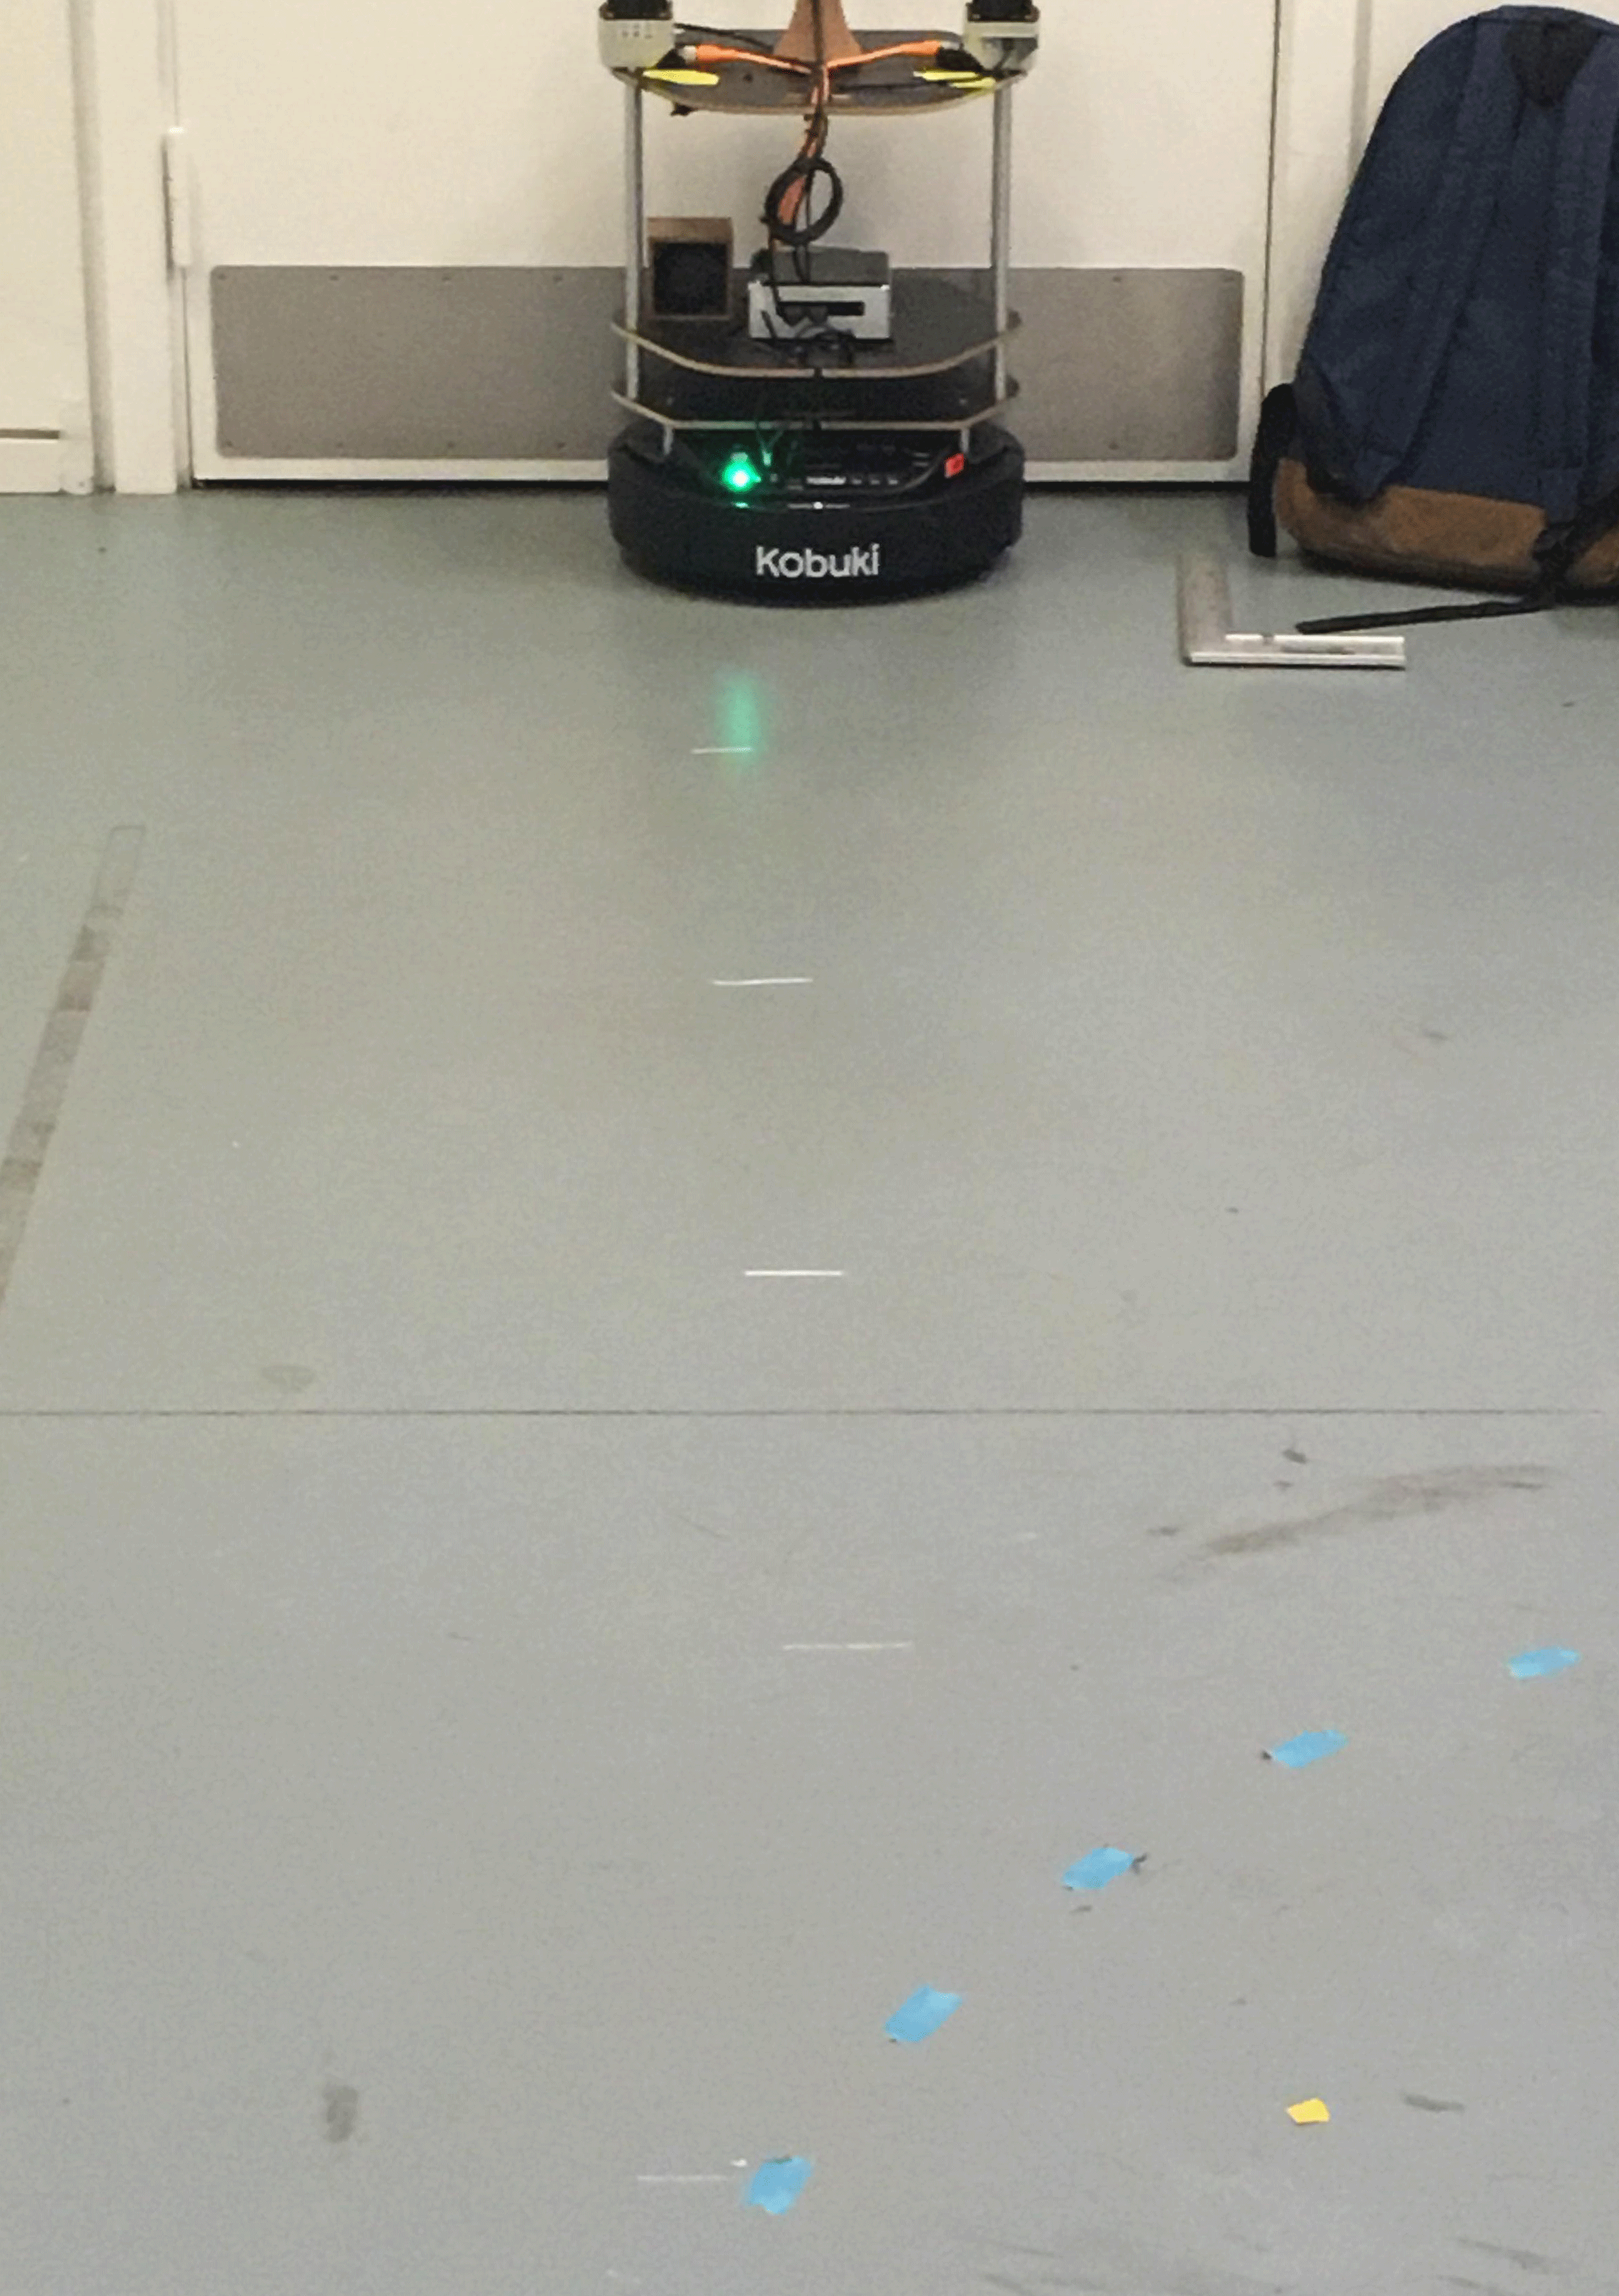
\includegraphics[width=0.75\textwidth]{figures/AccuracySetup2.png}
%     \caption{The position of the robot and LIDAR, with white chalk lines marking the distance to the LIDAR, if it was placed on the floor. This was done as it is difficult to mark distances at the same height as the LIDAR.}
%     \label{fig:AccuracySetup2}
% \end{figure}


\textbf{Execution}: Person A held the piece of cardboard at the marked distances, starting from 0.5m all the way to 4.5m at 0.5m increments. When person A thought the cardboard was placed at the exact marked spot and held vertically, he let person B know, who then denoted the distance read from the LIDAR. Person B only denoted the distance when person A told him to, to achieve the best distance. Person A was fiddling the cardboard when placing on the chalk line, and Person A knows when the board is in the right place.\\
Person B would look at the stream of distance data and take the average of the next three incoming data lines, see figure \ref{fig:AccuracySetup3}. The smallest distance measured by the LIDAR was published, hence why it was important to use a small angle in an empty room. person B would also look at the program RViz, which was also used on the sideline to make sure nothing else was causing readings, other than the cardboard.\\

% \begin{figure}[H]
%     \centering
%     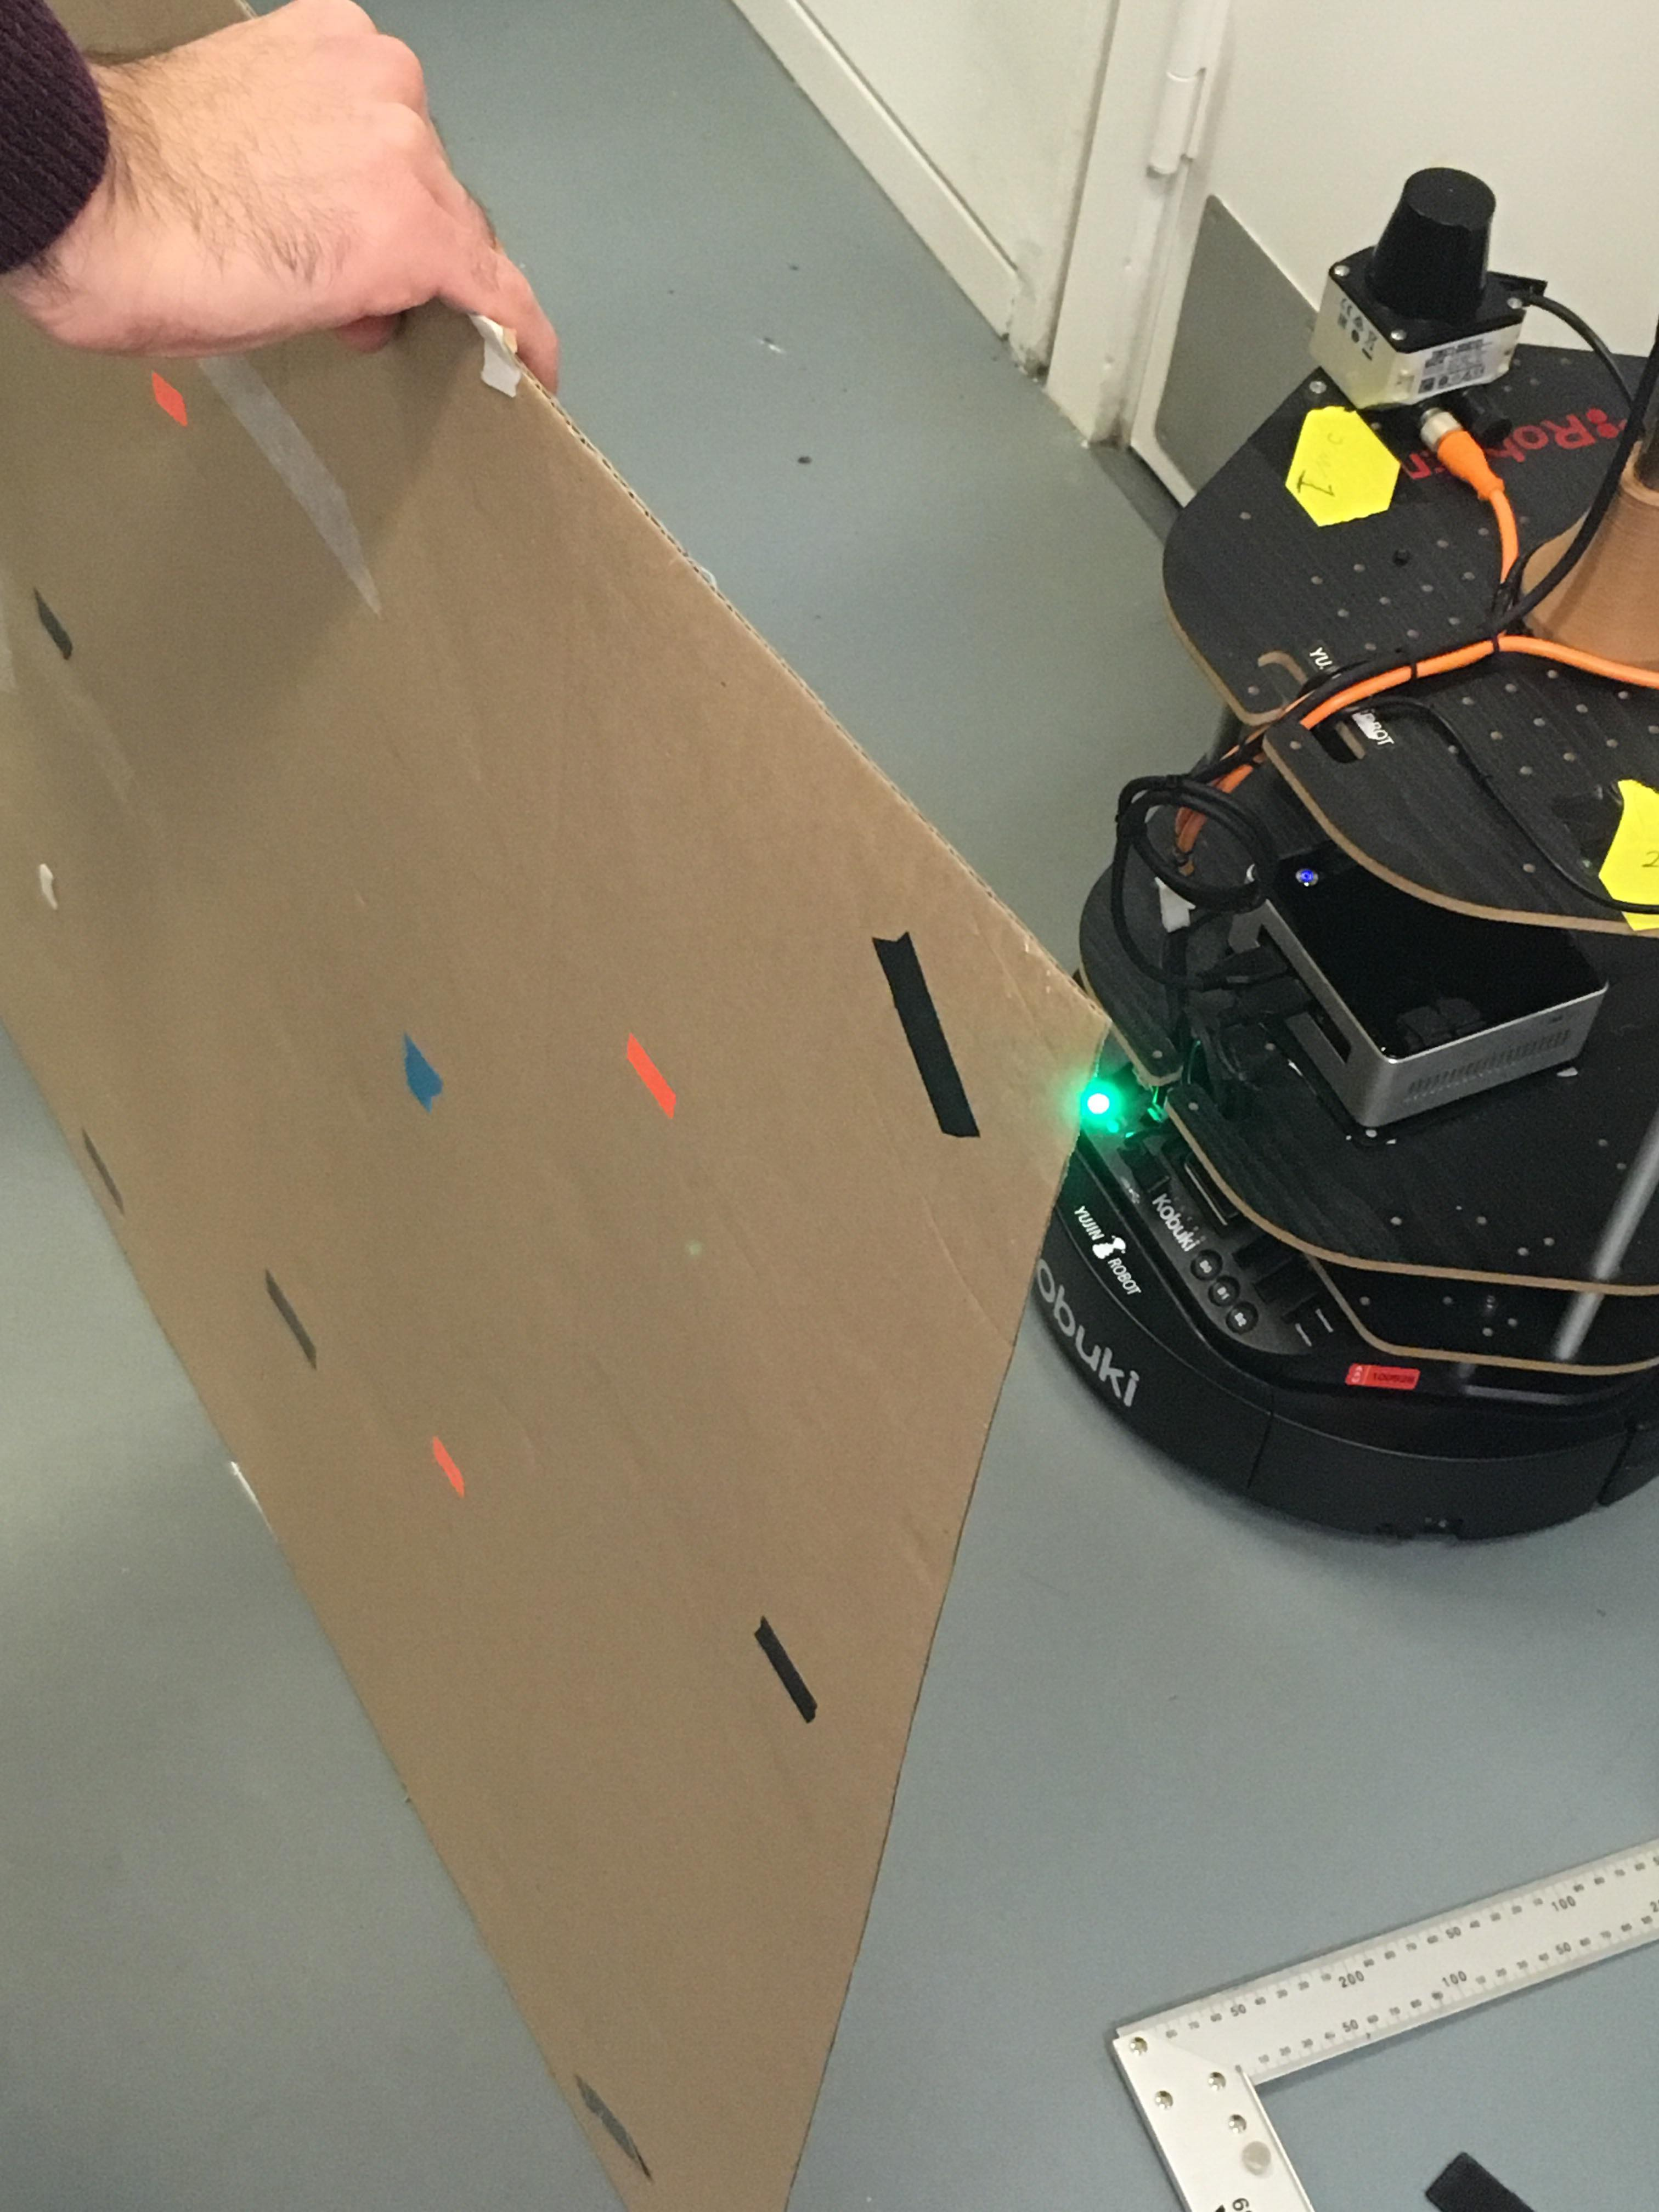
\includegraphics[width=0.45\textwidth]{figures/AccuracySetup1.jpg}
%     \caption{Person A holding the cardboard piece at the 0.5m point. The white chalk is barely visible at the bottom of the board.}
%     \label{fig:AccuracySetup1}
% \end{figure}

\textbf{Test Parameters}: The incoming data stream from the LIDAR for each distance from the cardboard to the LIDAR. Only 2 decimals were used, as from the third decimal, were changing too quickly to read. 

\begin{figure}[H]
    \centering
    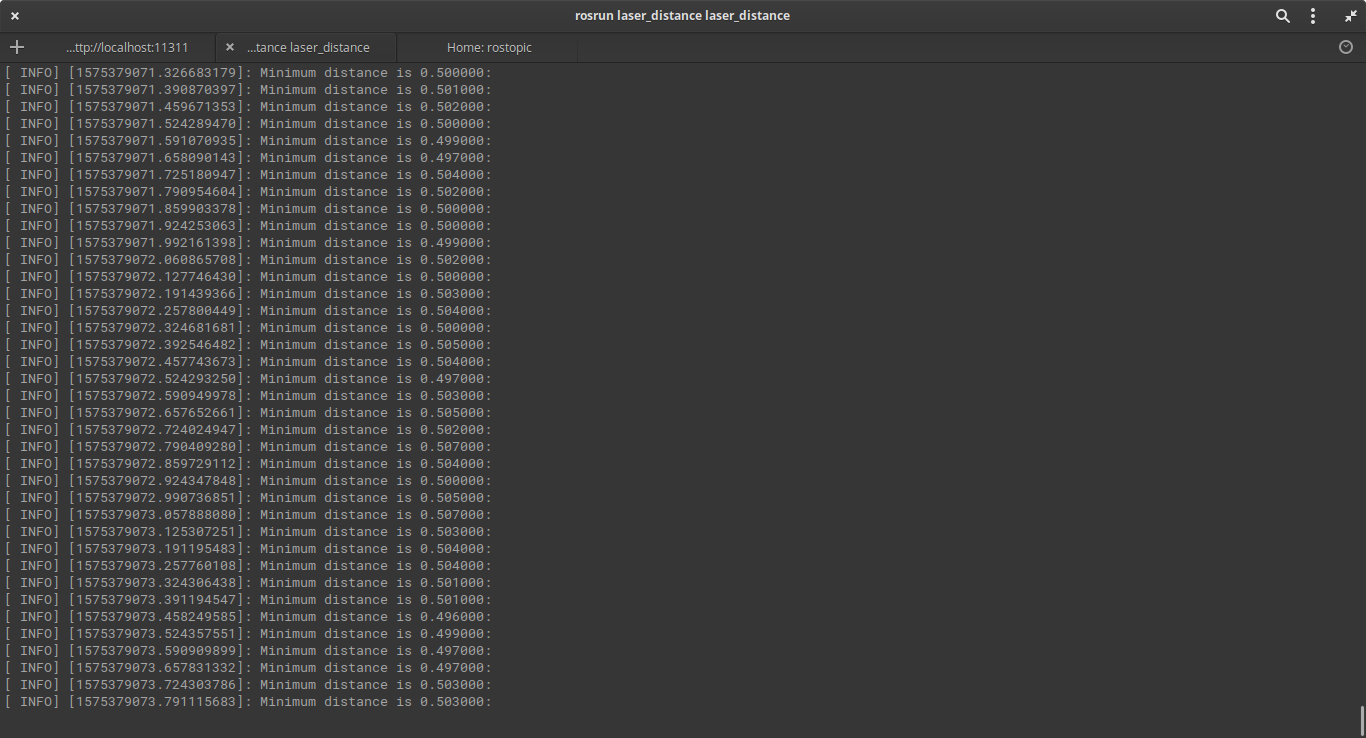
\includegraphics[width=1\textwidth]{figures/AccuracySetup3.png}
    \caption{The software that streamed the shortest distance read by the LIDAR. Person B used this to determine the distance, when person A said he was in position with the cardboard.}
    \label{fig:AccuracySetup3}
\end{figure}

\textbf{Results and analysis}:
\begin{center}
 \begin{tabular}{||c c c||} 
 \hline
 Marked distance & Measured Distance & Error percentage \\ [0.5ex] 
 \hline\hline
 0.5m & 0.5m & 0\%\\ 
 \hline
 1m & 1m & 0\%\\
 \hline
 1.5m & 1.49m & 1\%\\
 \hline
 2m & 2m & 0\%\\
 \hline
 2.5m & 2.51m & 0.4\%\\
 \hline
 3m & 3.02m & 0.6\%\\
 \hline
 3.5m & 3.5m & 0\%\\
 \hline
 4m & 4.01m & 0.2\%\\
 \hline
 4.5m & 4.5 & 0\%\\ [1ex] 
 \hline
 \label{table12}
\end{tabular}
\end{center}
Table \ref{table12} shows the results of the accuracy test. The error percentage averages 0.22\% throughout 9 readings at distances from 0.5m to 4.5m. This is so small it is not only irrelevant but points towards imperfections with the test setup. As the distance markings were done by hand, with measuring equipment, there is a chance of inaccuracies. Same goes for holding the cardboard at the exact mark and the right angle. The error margin of the error is 20mm according to SICK themselves.\\ %REF here

\textbf{Sources of error}:
\begin{itemize}
    \item The SICK TiM571 LIDAR has an error margin of 20mm.\cite{timerrormargin}
    \item The cardboard was held by hand, and might not be held in the correct angle at all times. Small movements would be caught on the readings and may be the reason for the average result be a little incorrect.
    \item The chalk lines on the floor have been drawn manually and there may have been a slight movement when drawing the lines, making a small mistake in where the cardboard would be placed when doing the readings.
\end{itemize}

\section{Leg detection test}
%This test serves to gain knowledge about the reliability of the leg detection system used for this robot. 
This test serves to gain knowledge about the reliability of how the LIDARS work with the software written for the leg detection. It is important to know the capabilities and limits of a system, especially when moving a robot in dynamic environments with humans. It was also used to decide whether one LIDAR detecting a person is enough or if both LIDARs need to confirm it simultaneously within a 1cm devation between the LIDARs.\\


\textbf{Equipment}: The equipment used when conducting this test consists of two Sick TIM571 LIDARs, ROS People's package, a room with 5 meters * 5 meters grid marked on the floor and two test persons.\\

\textbf{Setup}: The robot is located in the corner of the 5m*5m grid marked on the floor, angled towards the diagonally opposite corner, see figure \ref{fig:LidarCoverage}. 

\begin{figure}[H]
    \centering
    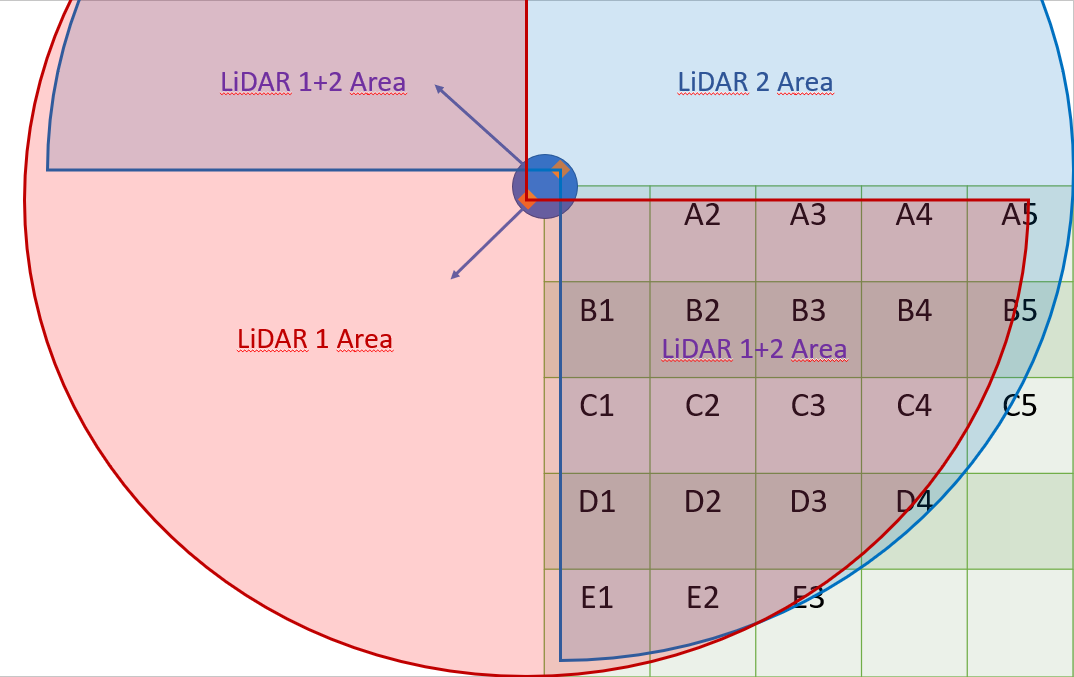
\includegraphics[width=0.85\textwidth]{figures/LidarCoverage.png}
    \caption{A visual representation of the LIDARs covered area when limited to 5m.}
    \label{fig:LidarCoverage}
\end{figure}

This is because the space in a 90 degrees angle behind the robot is what we are most interested in using to detect people. Test persons will take turns standing twice, with two different poses, in specific quadrants and the person detection will be noted (false or positive). The layout is shown in figure \ref{fig:LidarCoverage} and \ref{fig:LegDetectorSetup}. 

\begin{figure}[H]
    \centering
    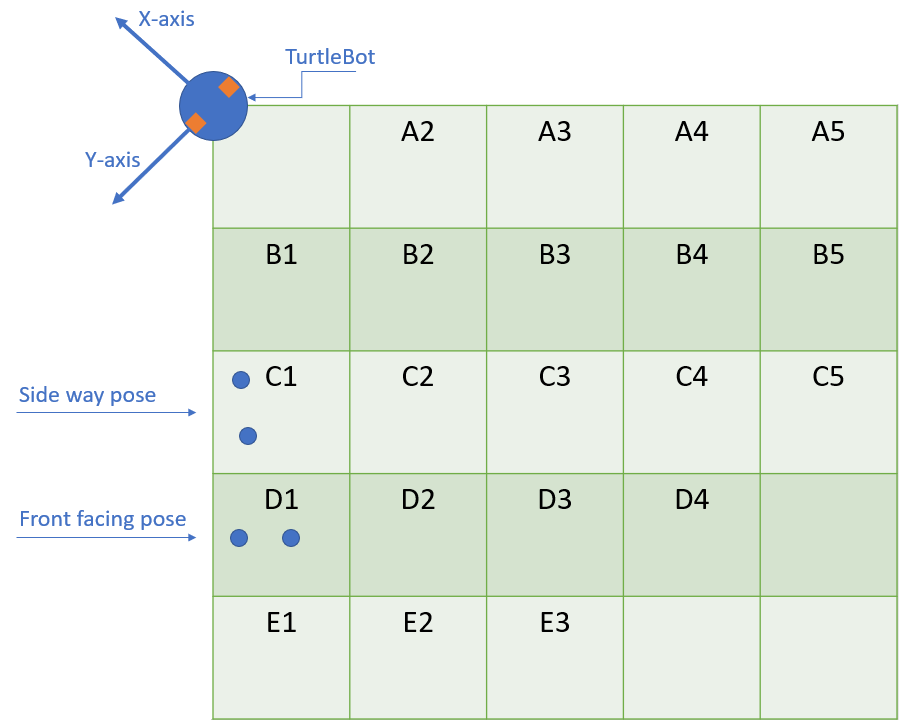
\includegraphics[width=0.85\textwidth]{figures/LegDetectorSetup.png}
    \caption{A design of the layout of the test setup.}
    \label{fig:LegDetectorSetup}
\end{figure}

Since the robot is placed in a corner full of windows, the curtains were used to eliminate laser reflection from the glass, however, it turned out that the curtain drapes look like human legs, so $1.2m^2$ portable blackboards were used to shut off reflections and false positives from the curtain drapes, as shown in figure \ref{fig:testfront} and \ref{fig:testside}.\\

\textbf{Execution}: This will be tested with two people, test person A and test person B. Each test person will stand in a quadrant, see figure \ref{fig:LegDetectorSetup}, with a front facing pose, see figure \ref{fig:testfront}, then do a side way pose, see figure \ref{fig:testside} and then proceed to the next quadrant, all the way through the whole grid. E4, E5 and D5 are excluded due to the range limit implemented in the software and thus will distort the data. A1 is excluded as no person should be able to get this close to the robot while it is guiding. The test will be done with both LIDARs needing to confirm the presence of legs and once more with only one LIDAR having to confirm it, here on referred to as single or double LIDAR confirmation.\\

\begin{figure}[H]
    \centering
    \begin{minipage}[b]{0.48\linewidth}
    \centering
    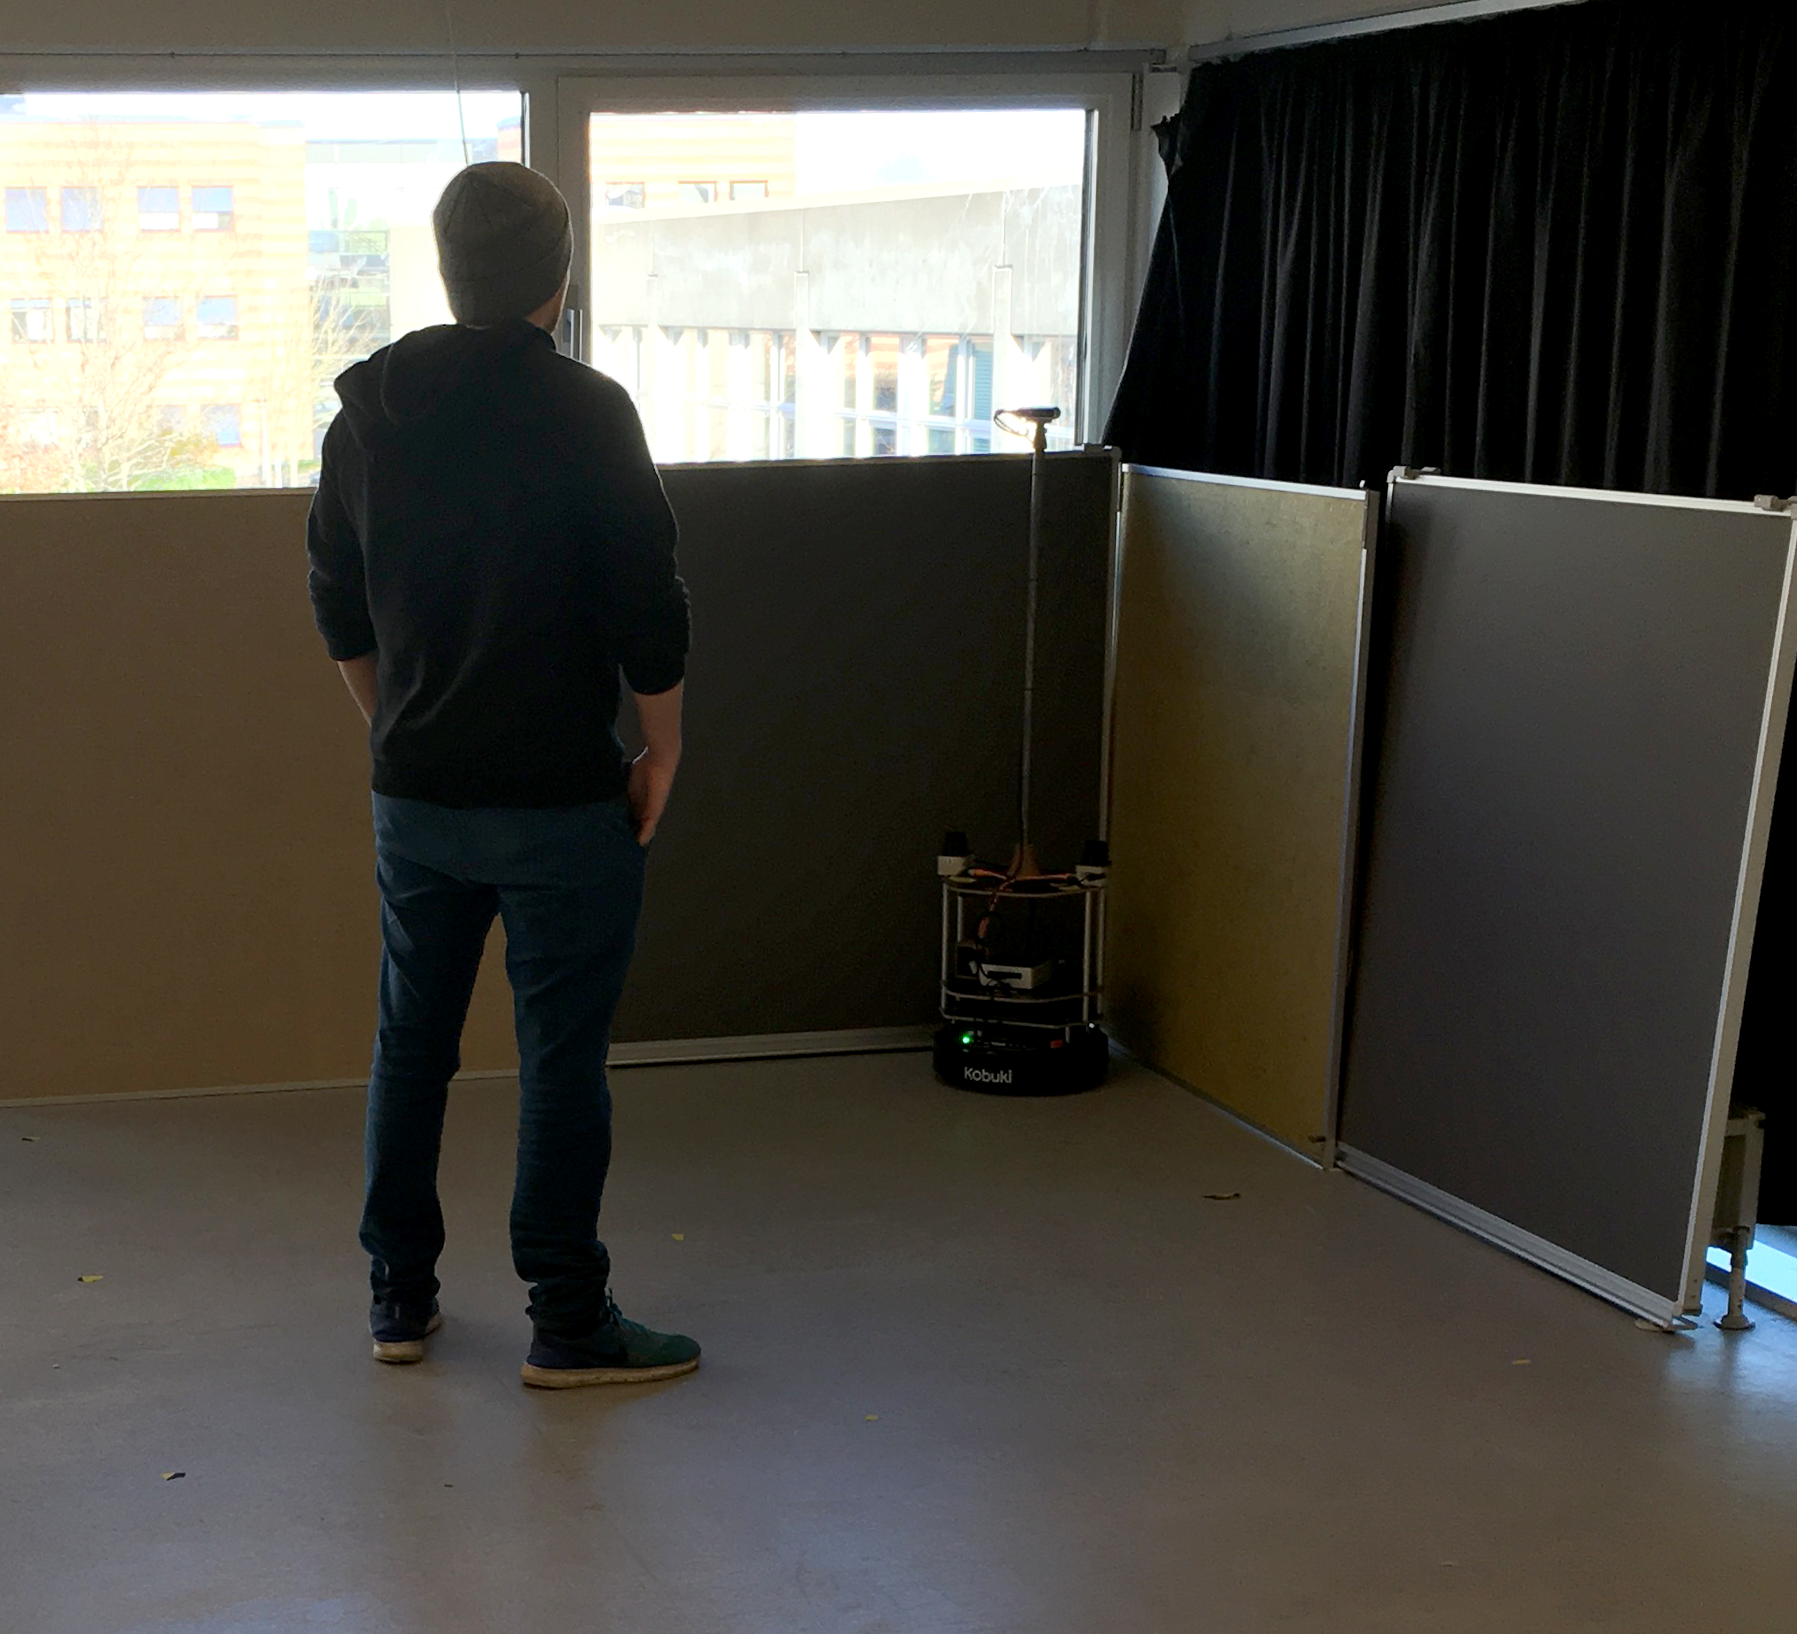
\includegraphics[width=\textwidth]{figures/test_front.png}
    \caption{Test person B with a front facing pose, relative to the robot.}
    \label{fig:testfront}
    \end{minipage}
    \hspace{0.2cm}
    \begin{minipage}[b]{0.48\linewidth}
    \centering
    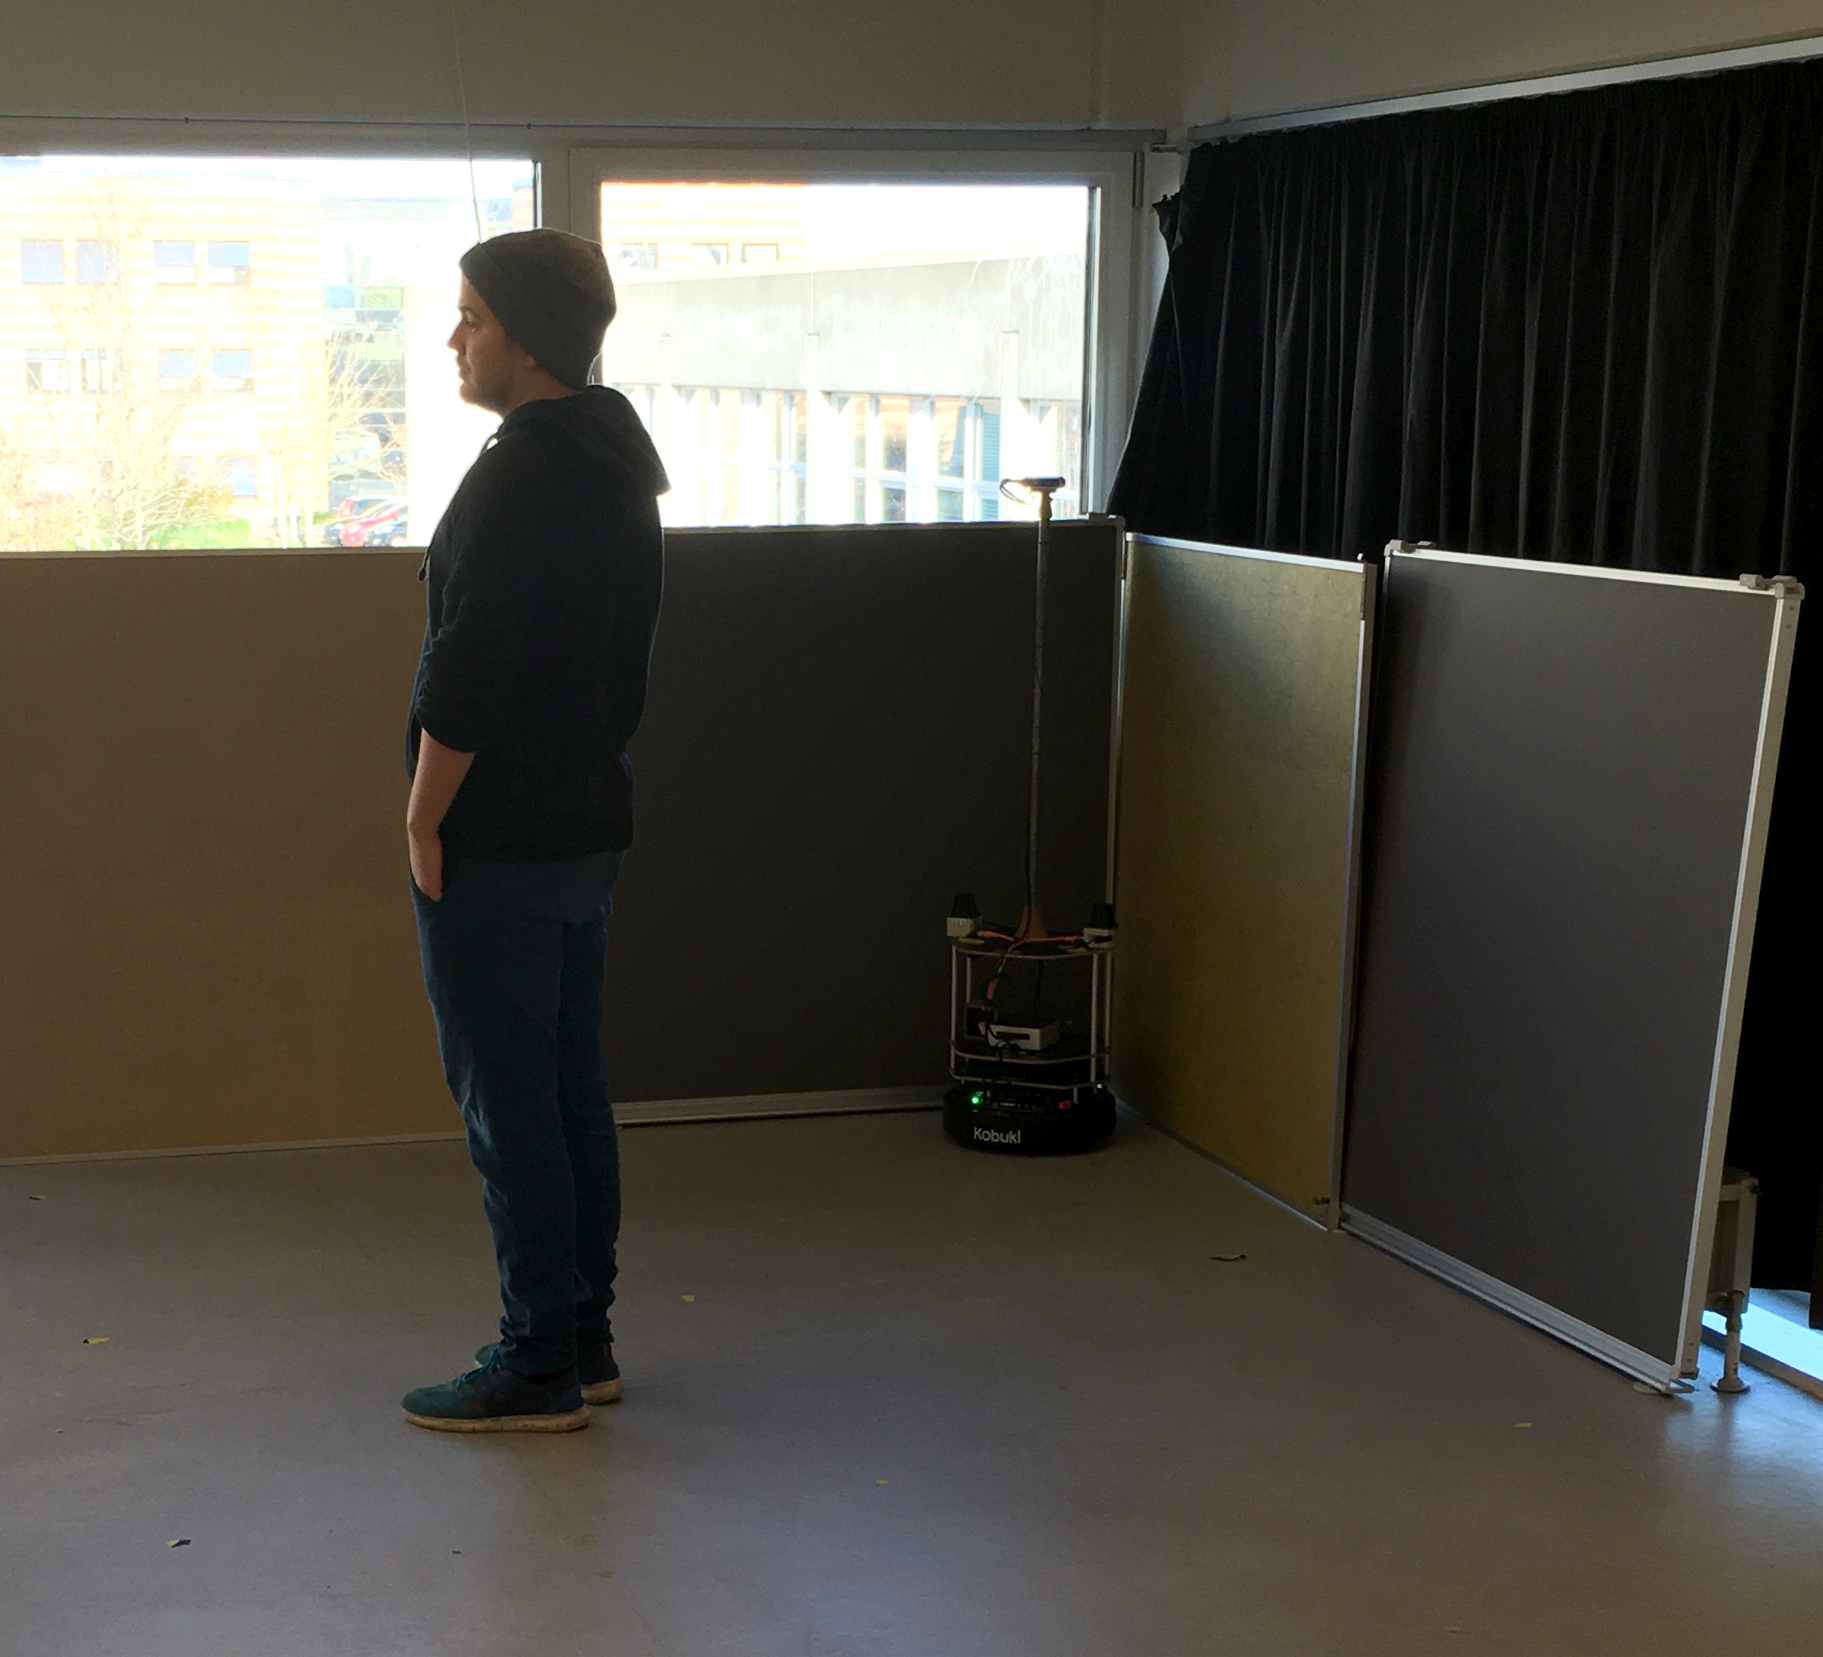
\includegraphics[width=\textwidth]{figures/test_side.png}
    \caption{Test person B with a side way pose toward the robot.}
    \label{fig:testside}
    \end{minipage}
\end{figure}

\textbf{Test parameters}: The software will stream continuous data if the LIDAR(s) detect a person. To accept that a person is detected, at least 2 seconds of full data must be streamed within the first 4 seconds of test person A/B moving to the quadrant.\\

\textbf{Results and analysis}:
As the results are from two different persons wearing different coloured pants on different days, we will first argue whether or not the data can be treated as one set or it should be separated by test person. Looking at figure \ref{fig:CombinedLegDetector}, it is visible that the difference between the 4 parameter readings ranges from 14\% to 5\%. This is deemed small enough for the data to be treated as one set and will from now on be treated as such, as it is similar enough to not separate them. Had the difference from person A and B been significant, perhaps more tests should be done to conclude why the difference would be so large and whether or not the data could be used a single set.\\

\begin{figure}[H]
    \centering
    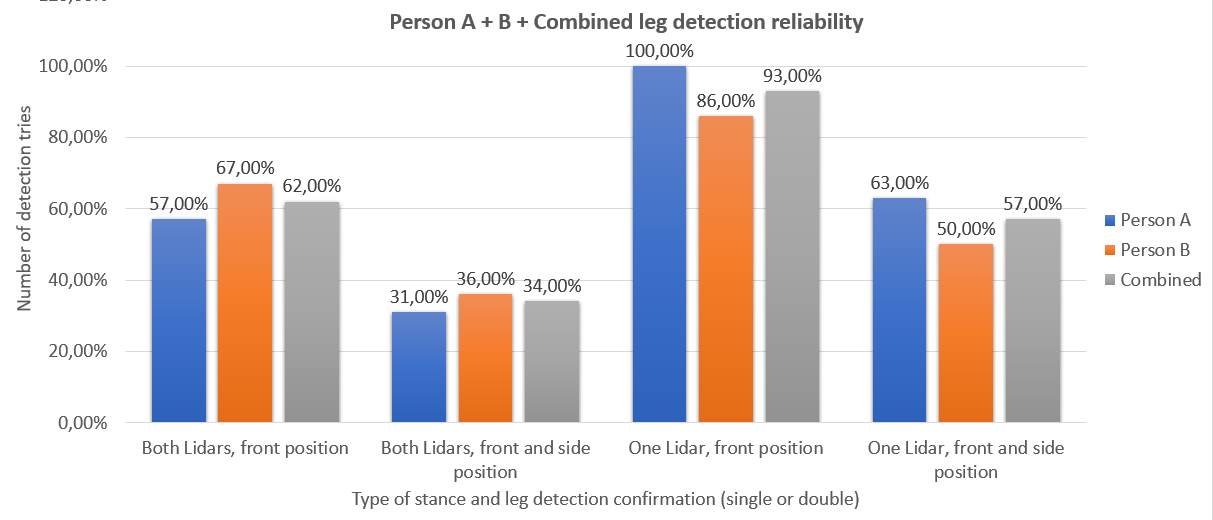
\includegraphics[width=1\textwidth]{figures/CombinedLegDetector.png}
    \caption{A graph showing the success rate between different test persons and the success rate of both persons combined, with the intention of combining or separating the data sets.}
    \label{fig:CombinedLegDetector}
\end{figure}

The leg detection was conducted with both a front face position and a side way position, however the success rate in correctly detecting legs dropped from 62\% to 5\% with double LIDAR confirmation and from 93\% to 21\% with single LIDAR confirmation, see figure \ref{fig:CombinedLegDetection2}. We will exclude the side way position for now, as we are only interested in detection the person(s) following the robot when it is guiding a user, and the user(s) is/are highly unlikely to follow it by walking sideways. Customers may do a side way stance when launching the guide feature and when picking up an item from the shelf, however this prototype focuses on the guiding part and as a prototype will not deal with that for now.

\begin{figure}[H]
    \centering
    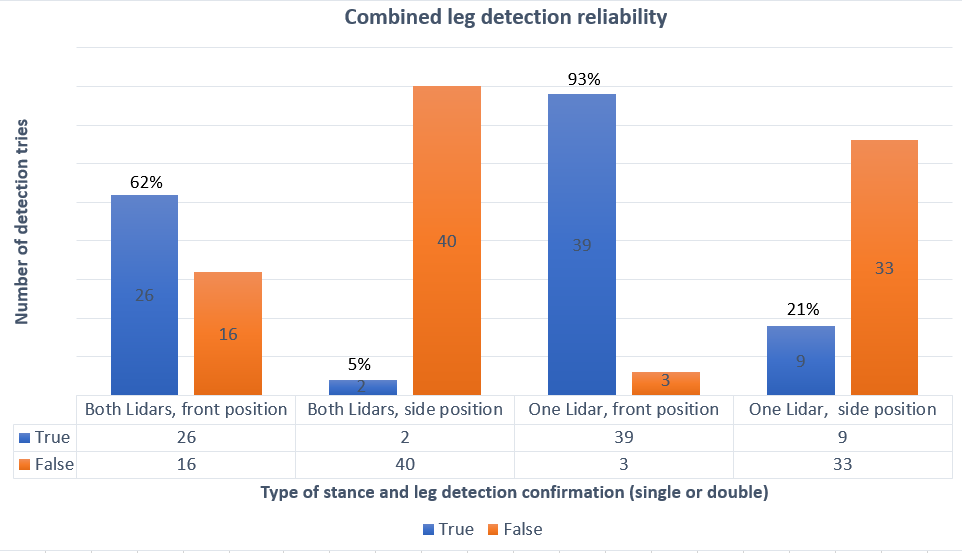
\includegraphics[width=\textwidth]{figures/CombinedLegDetection2.png}
    \caption{A graph depicting success rate with relation to the persons stance.}
    \label{fig:CombinedLegDetection2}
\end{figure}

Looking at figure \ref{fig:LidarCoveragePercentage}, it shows how the success rate of the system seems to diminish in row D and E. As column 4 and 5 are as far away, it seems unlikely that it is due to distance. The room in which the test was performed, only had curtains that covered rows A, B and C. Figure \ref{fig:FigureLightPolltuion} shows how light pollution may have had an affect on the success rate, as the rows affected by the light have decreased success rate.

\begin{figure}[H]
    \centering
    \begin{minipage}[b]{0.48\linewidth}
    \centering
    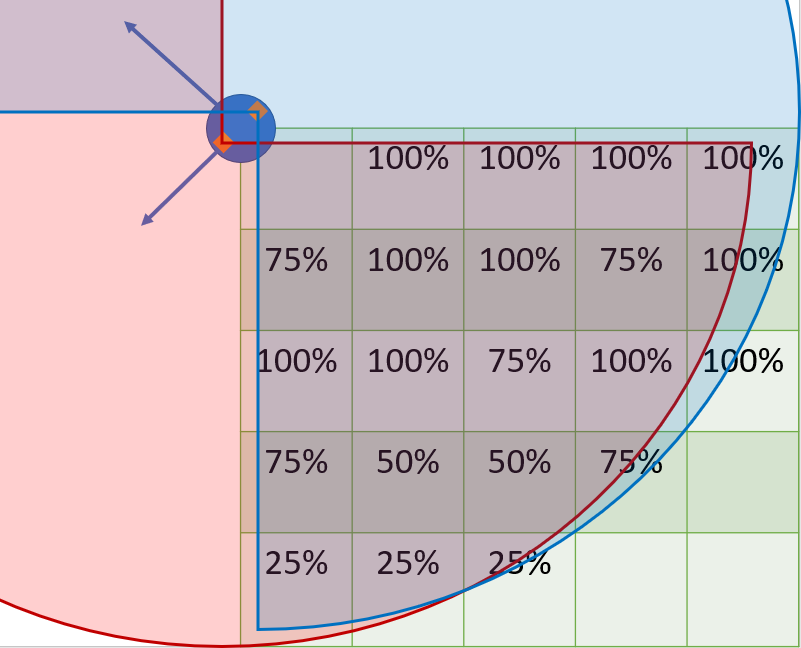
\includegraphics[width=\textwidth]{figures/LidarCoveragePercentage2.png}
    \caption{The success rate in percentage related to quadrant position.}
    \label{fig:LidarCoveragePercentage}
    \end{minipage}
    \hspace{0.2cm}
    \begin{minipage}[b]{0.48\linewidth}
    \centering
    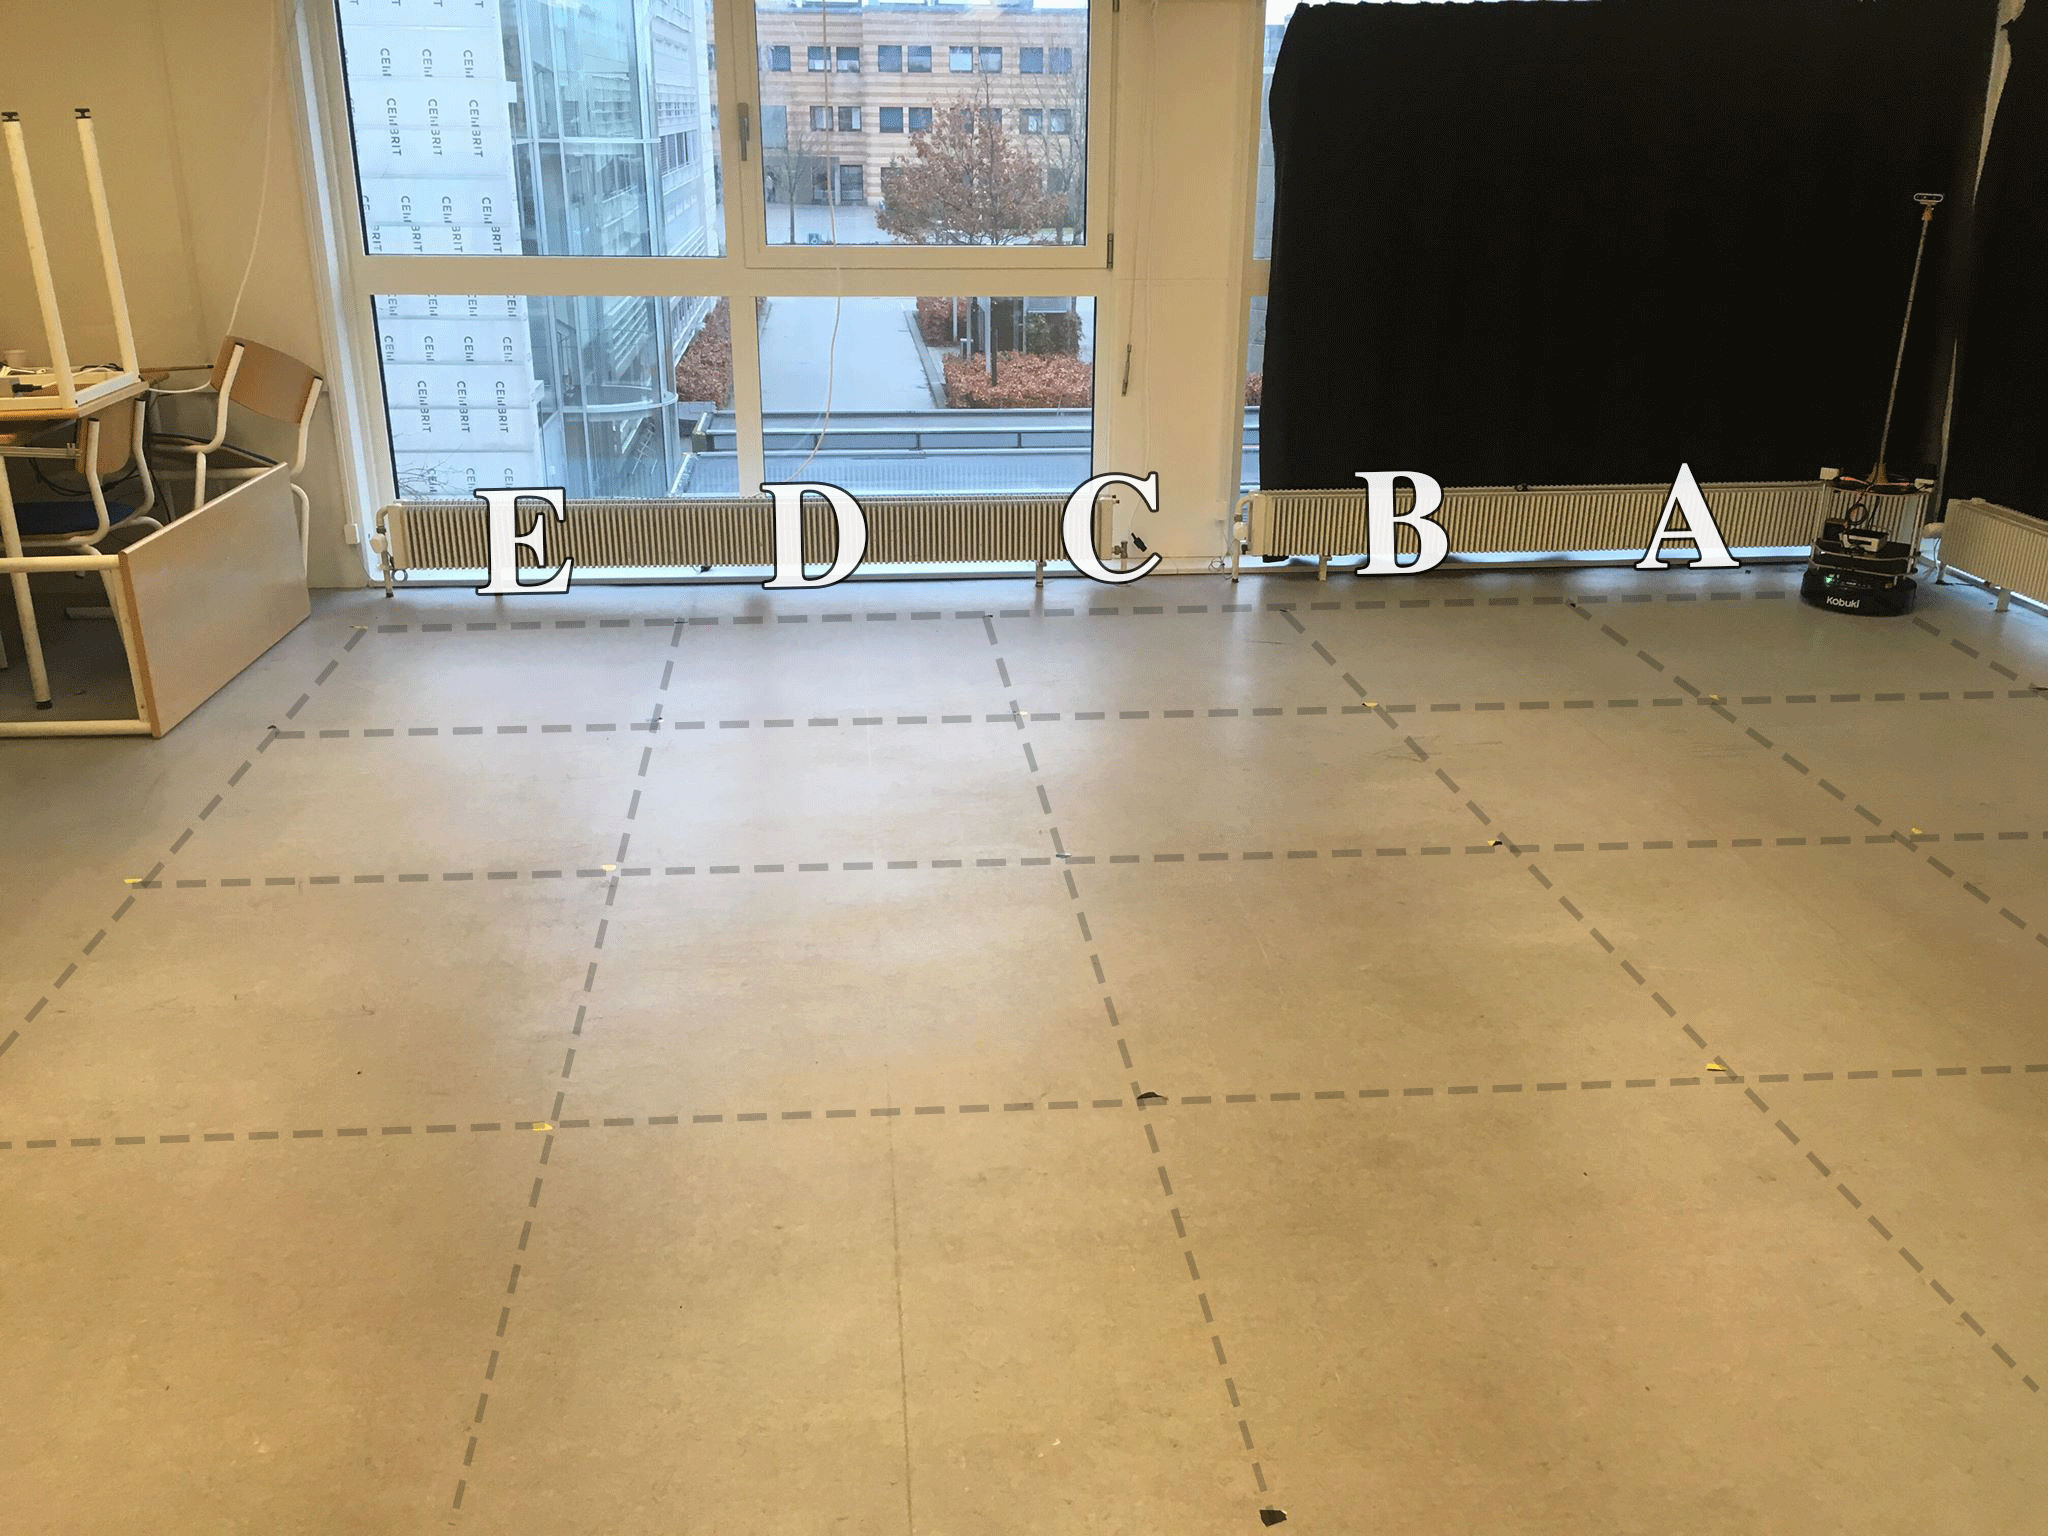
\includegraphics[width=\textwidth]{figures/FigureLightPollution_nr.png}
    \caption{A picture of the test location, emphasising that light breached into the room, illuminating rows D and E.}
    \label{fig:FigureLightPolltuion}
    \end{minipage}
\end{figure}

\textbf{Sources of error}:
A bit of movement from the test person can eliminate many false negatives. The test person had to be standing still before the data stream was counted, but when following a robot, movement is of course necessary. Almost all of the false negative readings started streaming data when the test person walked towards the next quadrant.\\

Illumination of the test room also seemed to have an impact on the results. Whether it is a sudden change in illumination, the type of light or a reflection caused by the light can not be confirmed by the test.\\

The test room was empty when testing, to only focus on testing the leg detection without other disturbances. This is not a realistic dynamic environment for the robot to move around in and must be considered when designing the full system. A table and a chair was put inside the testing environment to see if it would mistake table and chair legs for human legs. The leg detection did not detect things as persons. This was important to test as the double confirmation LIDAR setup likely would have caused a lower success rate but would rule out more false positives. This is because persons can only be detected in the area that both LIDARs cover, as seen in figure \ref{fig:LidarCoverage}. In the area that is shared by both LIDARs, both the LIDARs would need to have line of sight of the person in question to detect a person. The single confirmation setup would likely increase success rate, as only one of the LIDARs would need a clear line of sight, but perhaps at the cost of more false positives. Even with single LIDAR setup, the tables and chairs were not mistakenly seen as persons. Figure \ref{fig:SetupTableChair} shows a table and a chair being inside the testing environment, to confirm whether a single confirm setup would lead to more false positives or not.\\

\begin{figure}[H]
    \centering
    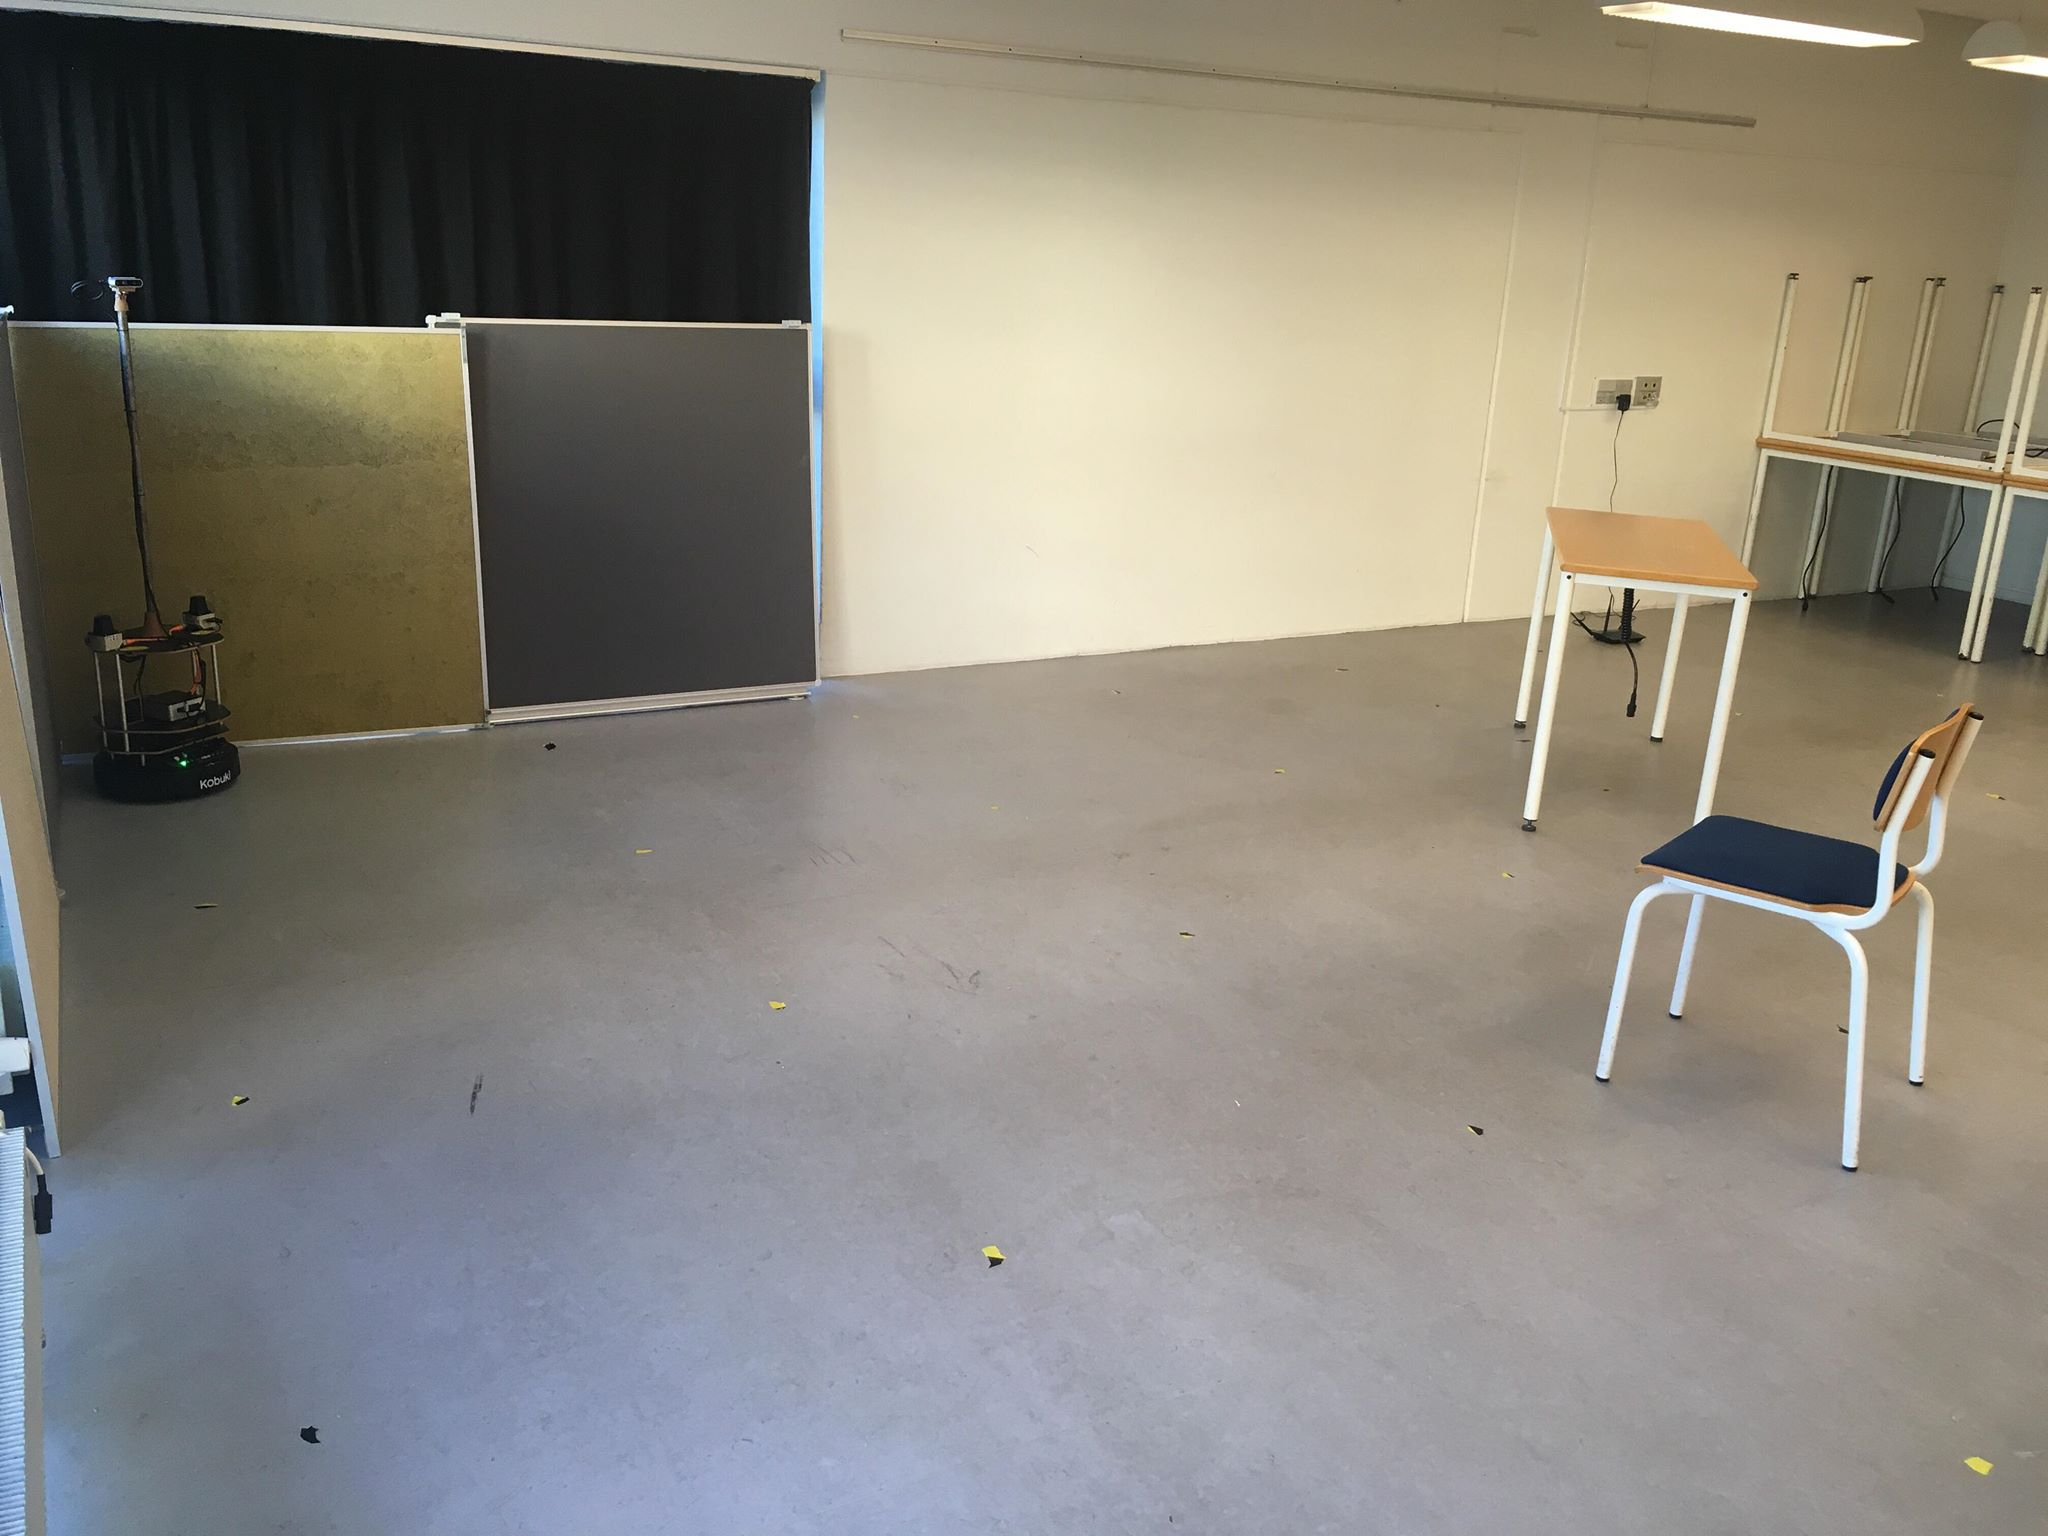
\includegraphics[width=0.75\textwidth]{figures/SetupTableChair.jpg}
    \caption{A picture of the environment setup with a table and a chair to see if the table and chair legs would be detected as persons.}
    \label{fig:SetupTableChair}
\end{figure}

\section{Face ID test}
The performance of the Face ID will affect the overall system and is therefore highly relevant to test on its own. How often it works, how distance, different light settings, different faces and other factors change the success rate.\\
Reliability\\
Sensor precision\\


\textbf{Equipment}:
\\
\textbf{Setup}:
\\
\textbf{Test parameters}:
\\
\textbf{Results and analysis}:
\\
\textbf{Sources of error}:

\section{Kalman filter test}
The Kalman filter test will consist mainly of a before and after test of the components we add the filter to, to see the difference.\\
Performance with filter.\\
Performance without filter.\\

\textbf{Equipment}:
\\
\textbf{Setup}:
\\
\textbf{Test parameters}:
\\
\textbf{Results and analysis}:
\\
\textbf{Sources of error}:

\section{Velocity controller test}
A velocity tests has been done to prove that the velocity changes dependant to the distance from a person to the robot. When the distance is 1.2m the velocity should be at its highest and when the distance is close to 3m, the velocity should decrease to minimum and stop. This tests also shows whether or not the velocity is the value it has been programmed to be for the specific distances.\\

\textbf{Equipment}: The equipment used for executing the test is chalk to mark two lines, the robot used to move from one place to another and a timer.\\

\begin{figure}[H]
    \centering
    \begin{minipage}[b]{0.57\linewidth}
        \textbf{Setup}: The test is executed in a hallway where a goal line has been marked 4 meters from the start line, see figure \ref{fig:test_velocity_setup}.
        The robot is placed a bit before the start line and has to move across the goal line. The two lines has been marked on the floor with chalk and has to be clear to see for us to be able to determine when the robot has passed the line.\\
        
        \textbf{Execution}: Beginning the test, we tell the program what the distance from the robot to the human is. There is no actual human needed for following the robot in this test, since the program is told that there is one and with this static distance, a specific time is predicted as a result. When the distance is set to 1.2m, the robot is expected to have a velocity of 0.704m/sec. When the distance is set to 1.3m, the robot is expected to have a velocity of 0.666m/sec. These velocities has been pre-programmed to a specific distance with an algorithm. %This test is to confirm that the velocity will drop when the distance from human to robot increases.
        
    \end{minipage}
    \hspace{0.2cm}
    \begin{minipage}[b]{0.4\linewidth}
        \centering
        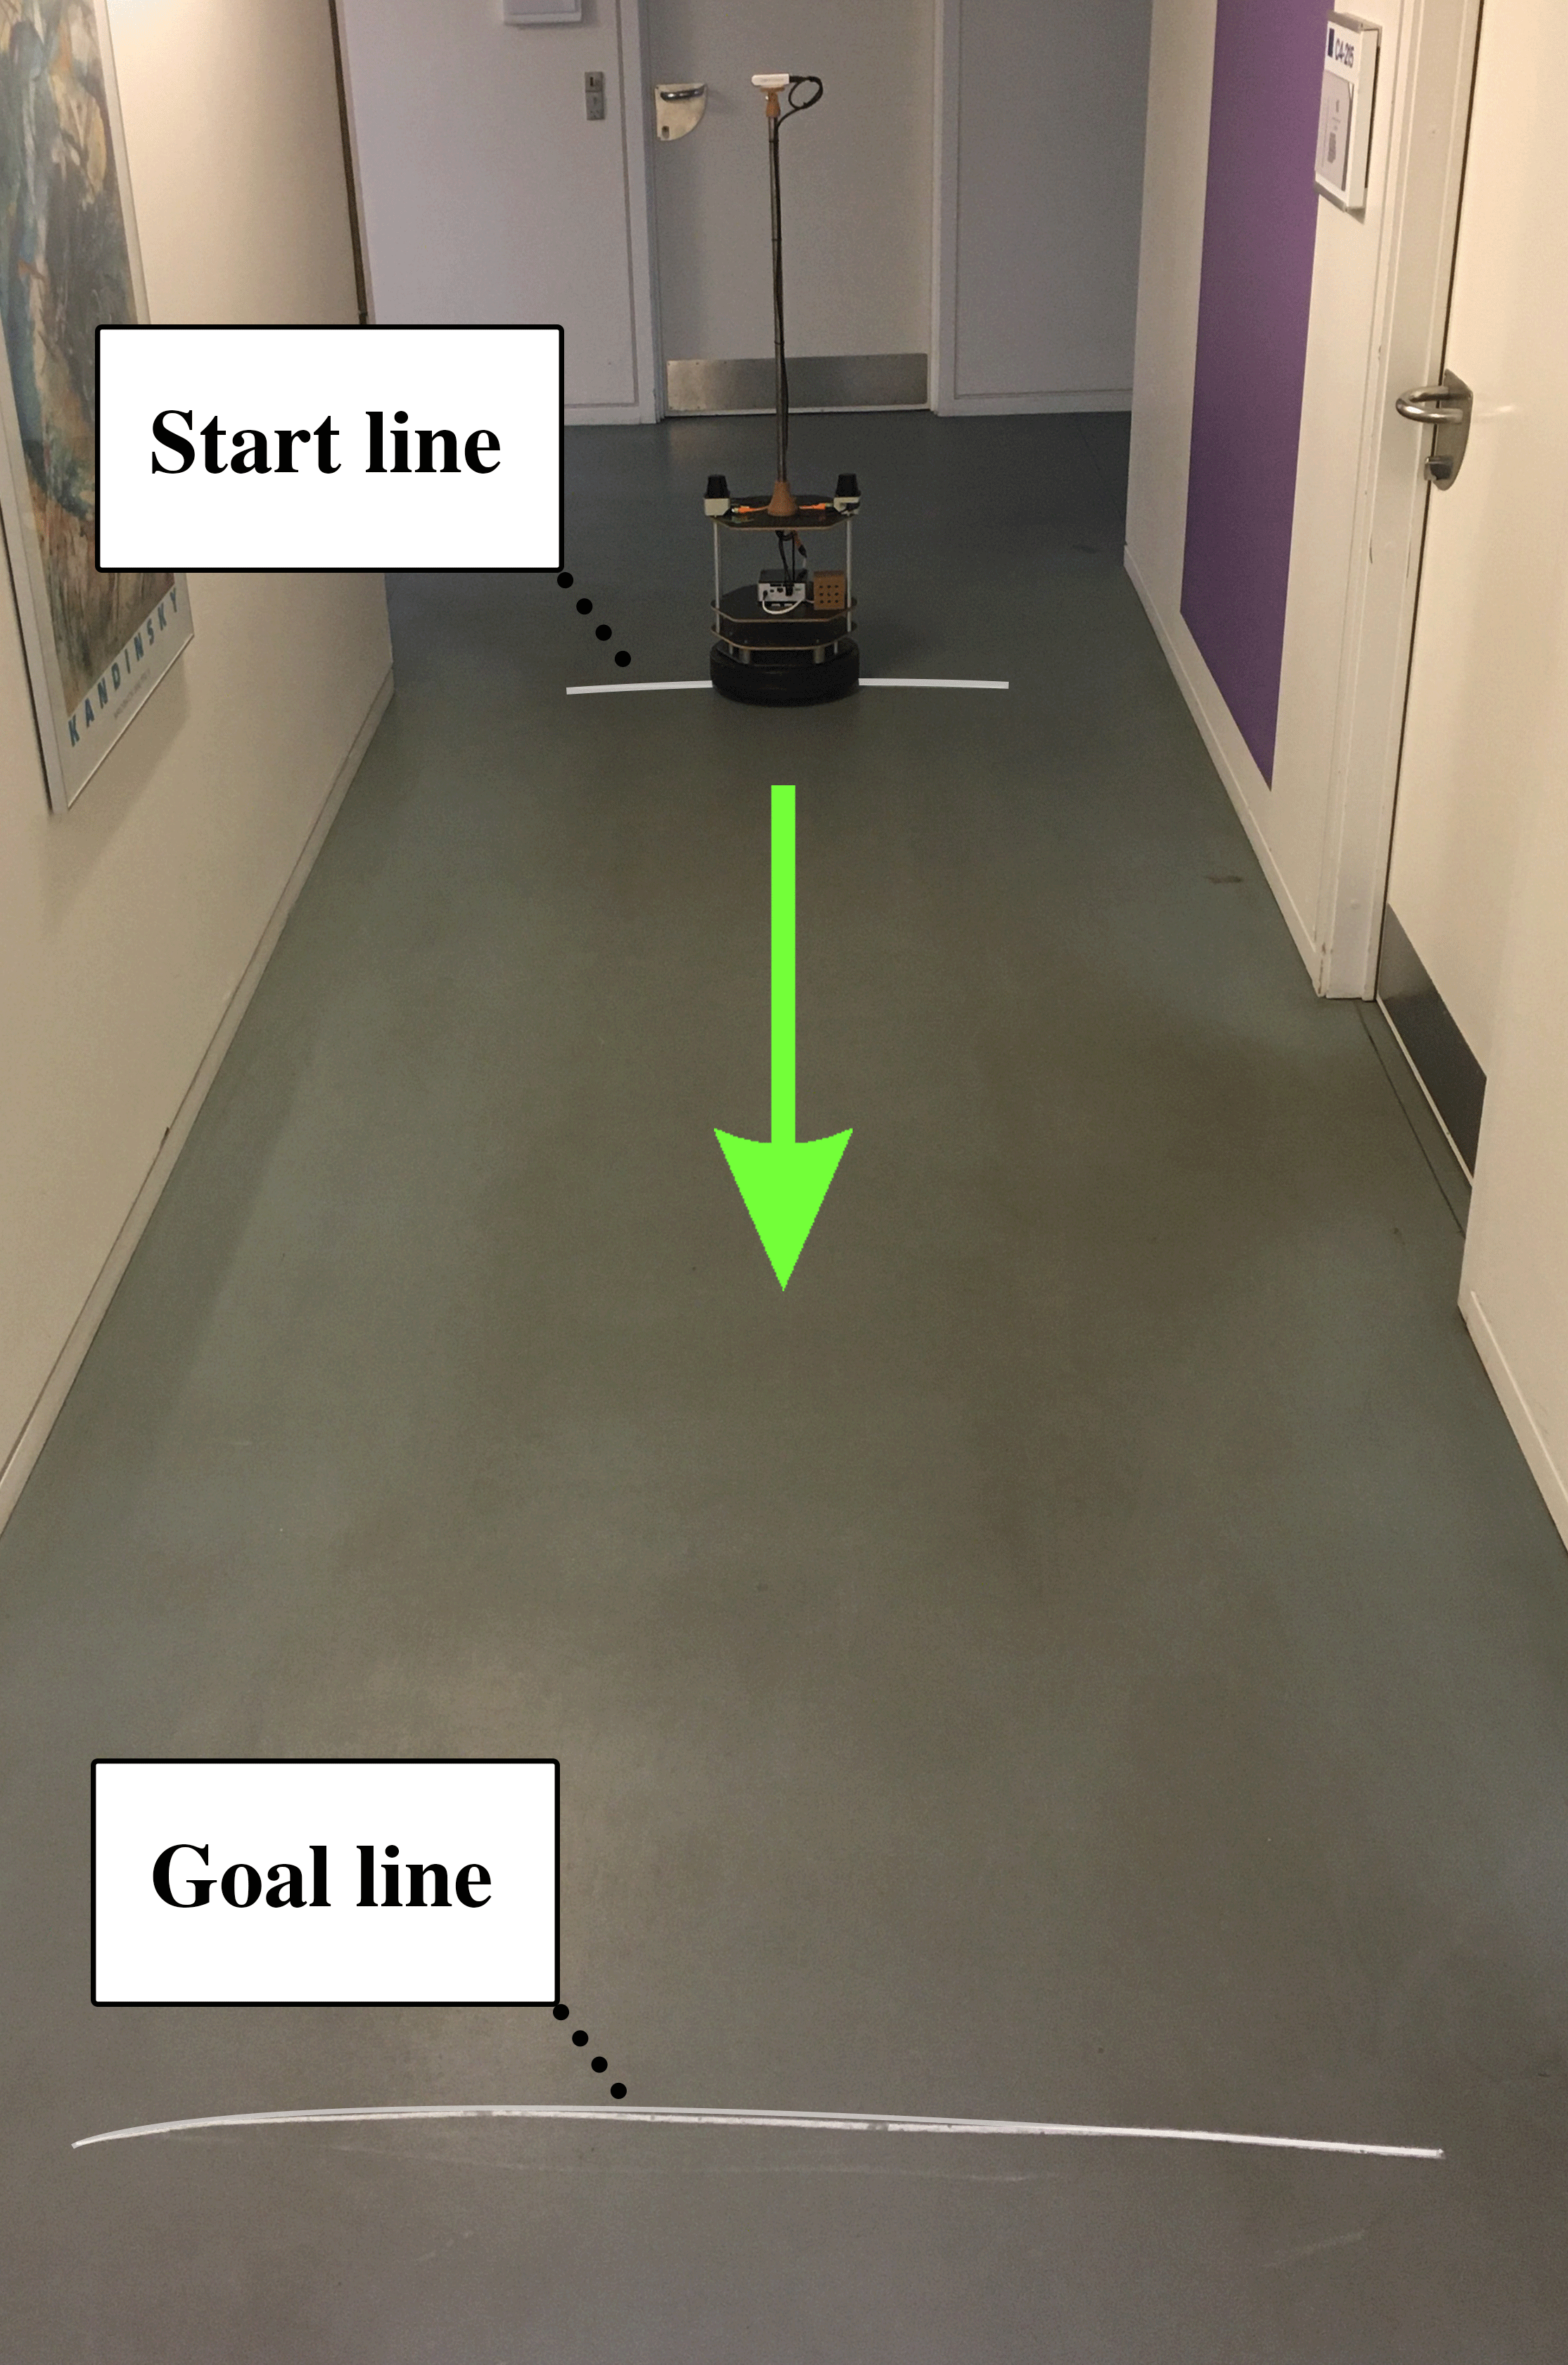
\includegraphics[width=\textwidth]{figures/velocityTest.png}
        \caption{Image showing the setup of the robot standing on the starting line ready to go to the goal line. There is 4 meters between the two marked lines.}
        \label{fig:test_velocity_setup}
    \end{minipage}
\end{figure}
The robot, which is placed a bit before the start line, is being told to move to a point across the goal line, via the software called RViz. When the robot's center crosses the start line, we manually start the timer and manually stop it as the center of the robot crosses the goal line. This has been done two times with ten different static distances to the robot. These different velocities can be seen on figure \ref{fig:test_velocity_setup}.\\

\textbf{Test parameters}: The time it takes for the robot to reach the goal line from the starting line, can be used for calculating if the velocity is behaving like wanted to in relation to the distance.\\

\textbf{Results and analysis}: Both the first and the second test result for all distances can be found in appendix \ref{} and the calculated average of the two can be seen on figure \ref{fig:TableVelocity}. \textit{Calculated distance} from the figure is calculated by \textit{Velocity}*\textit{Average time}, which is the distance it should have moved, if the given velocity was correct. Why the distance is more than 4m as it should not have been, is explained later under \textit{Sources of error}. \textit{Actual velocity} has been calculated by dividing the testing distance of 4m and the average time, such as $4/9.30=0.430$. This shows what velocity the robot actually had when moving.

\begin{figure}[H]
    \centering
    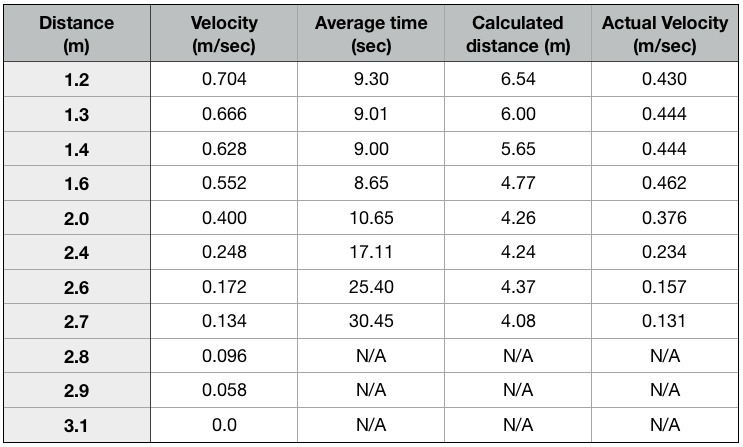
\includegraphics[width=\textwidth]{figures/velocity1.png}
    \caption{Results of the velocity test.}
    \label{fig:TableVelocity}
\end{figure}

When the distance was at its shortest of 1.2m, the velocity was at its highest, which should have been 0.704m/sec. Here the robot started to jiggle and could not keep up because of the hardware. When the distance was higher than 2.7m the robot started turning around itself very slowly and did not go forward, also because of the hardware. Since it could not move from the start line to the goal line, there are no result numbers for \textit{Average time}, \textit{Calculated distance} or \textit{Actual velocity} when the distance becomes too high.\\

\textbf{Sources of error}:
\begin{itemize}
    \item The distance between the two chalk lines are 4m $\pm 1cm$ and the imprecision may have affected the result.
    \item The timer was operated by a person and the response time of pushing the start/stop button may not have the highest precision and was also the reason for taking two tests of each distance.
    \item The payload of the robot was not considered when sending velocity commands and could have affected the time and is also one reason for the imprecision in \textit{Expected distance}.
    \item The floor surface could cause slippage of the wheels and as such it would take longer time to reach the 4m distance than expected.
    \item The reason for the robot to spin around itself could also be the payload of the robot was too high to move the robot with such a low given velocity.
\end{itemize}

\section{Full prototype test}
The prototype will be tested with all its components to see if they all work together as wanted and expected. Here a test will determine if all the tests above works at the same time with each other.


\textbf{Equipment}:
\\
\textbf{Setup}:
\\
\textbf{Test parameters}:
\\
\textbf{Results and analysis}:
\\
\textbf{Sources of error}:
